\documentclass[10pt]{article}
\usepackage[a4paper,margin=2cm]{geometry}
\usepackage{amsmath,amssymb,booktabs,enumitem,array,graphicx}
\usepackage[T1]{fontenc}\usepackage{lmodern}
\usepackage{pdflscape,tabularx,longtable}
\usepackage[font=small]{caption}\usepackage{placeins}
\setlength{\parindent}{0pt}\setlength{\parskip}{5pt}
\newcommand{\bs}{\beta^\star}\newcommand{\E}{\mathbb E}\newcommand{\asinh}{\operatorname{arcsinh}}\newcommand{\sk}{\sqrt k}
\newcommand{\Rf}{R_{\mathrm{full}}}\newcommand{\Ff}{F_{\mathrm{full}}}\newcommand{\dSh}{d_{\mathrm{Sh}}}
\newcommand{\step}[1]{\par\smallskip\textbf{Step #1.}\ }
\newcommand{\Part}[2]{\clearpage{\LARGE\bfseries Part #1.\ #2\par}\bigskip}
\title{Unlearning in diagonal linear networks:\\ setup, questions, derivations and results}
\author{}\date{25 November 2026}
\begin{document}\maketitle
We use a model in which the end point of every training run is known exactly, and ask two questions about gradient-based unlearning.
\textbf{(1)} Does it remove only the given samples (\emph{untraining}) or the whole distribution they came from (\emph{unlearning})?
\textbf{(2)} Is the forgotten behaviour deleted, or only hidden so that an attacker can recover it cheaply (\emph{tamper resistance})?

\textbf{How to read this.} Part I is the model and the data. Part II is the mechanism: how training moves the weights and where it stops, derived exactly (Sections~\ref{sec:flow}--\ref{sec:facts}; Section~\ref{sec:unbal} is optional). Part III states the unlearning losses and the two questions in terms of Part II. Part IV computes everything at large $d$ (replica and cavity). Part V has the results. Parts I--II are the core. One notation is used throughout; the table of symbols is in Section~\ref{sec:data}.
\tableofcontents

\Part{I}{Model and data}
\section{Model}
The network computes $f(x)=x^\top\beta$ with $\beta_j=u_j^+v_j^+-u_j^-v_j^-$; all weights start at the same value, which sets the initialisation scale $k$. Since $u_j^\pm=v_j^\pm$ at the start and this is preserved, $\beta=u^2-v^2$ entrywise with $u=u^+$, $v=u^-$; the derivations use this form. We assume gradient flow (full batch, small step) run until the training loss is zero. With true labels this is always possible, since $\beta^\star$ fits every sample.

\textbf{Implicit bias.} Training from a start $\beta_0$ on inputs $X$ (one column per sample) with targets $t$ ends at
\[
\operatorname*{argmin}_\beta\ D_{Q_k}(\beta,\beta_0)\quad\text{subject to}\quad X^\top\beta=t,
\qquad Q_k(\beta)=\textstyle\sum_jq_k(\beta_j),\quad q_k'(\beta)=\tfrac12\operatorname{arcsinh}\tfrac{2\beta}{\sqrt k},
\]
where $D_{Q_k}$ is the Bregman divergence of $Q_k$ (Woodworth et al.\ 2020; Azulay et al.\ 2021). Derived in Section~\ref{sec:ends}. Small $k$ favours sparse solutions (rich regime); large $k$ favours the smallest Euclidean change (lazy regime).

\textbf{Rescaling.} Multiplying all weights by $\sqrt\kappa$ maps $\beta\to\kappa\beta$ and $k\to\kappa^2k$ (Result 4).

\section{Data}\label{sec:data}
The $d$ input coordinates are split into three blocks: retain-only $d_R$, shared $\dSh$ and forget-only $d_F$. One sparse teacher labels all data: each entry of $\beta^\star$ is $\pm\rho^{-1/2}$ with probability $\rho/2$ each and $0$ otherwise, and $y=x^\top\beta^\star$ (no noise; the derivations allow $y=x^\top\beta^\star+\sigma\xi$, $\xi\sim\mathcal N(0,1)$). Block $B$ is a fraction $p_B$ of the coordinates. The two classes differ only in which coordinates their inputs use:
\[
P_R:\ x\sim\mathcal N(0,\tfrac1d I)\ \text{on } d_R\cup\dSh,\ \ 0 \text{ on } d_F;
\qquad
P_F:\ x\sim\mathcal N(0,\tfrac1d I)\ \text{on } \dSh\cup d_F,\ \ 0 \text{ on } d_R .
\]
We draw a retain set $\Rf$ of $n_R$ samples from $P_R$ and a forget set $\Ff$ of $n_F$ samples from $P_F$; the training data is $D=\Rf\cup\Ff$. The unlearner is given a retain set $R\subseteq\Rf$ (usually all of it) and a deletion request $F\subseteq\Ff$ (a random subset). All set sizes grow in proportion to $d$, and $d\to\infty$. The free parameters are the block proportions $|d_R|:|\dSh|:|d_F|$, the sample proportions $n_R/d$, $n_F/d$, $|R|/n_R$, $|F|/n_F$, the sparsity $\rho$, and the geometry $k$.

\textbf{What pretraining learns.} If $n_R\ge|d_R|+|\dSh|$, the retain data determine $\beta$ on $d_R\cup\dSh$, so $A(D)=\beta^\star$ there. On $d_F$, $A(D)=\beta^\star$ only above a learning threshold (about $0.51\,|d_F|$ forget samples in the rich regime at $\rho=0.2$, $|d_F|$ in the lazy regime); below it $A(D)$ is a wrong estimate.

Write $A(T)$ for the model trained from $0$ on a dataset $T$. The pretrained model is $A(D)$. The two reference models are
\begin{align*}
&A(D\setminus F) && \text{untraining reference: as if $F$ had never been seen;}\\
&A(D\setminus\Ff) && \text{unlearning reference: as if the forget class had never been seen.}
\end{align*}

\textbf{Metrics.} \emph{Retain error} and \emph{forget error}: $\mathbb E(x^\top\beta-x^\top\beta^\star)^2$ over fresh $x\sim P_R$ and $x\sim P_F$. \emph{Error on $F$} and \emph{on the kept forget samples}: mean of $(f_i-y_i)^2$ over $F$ and over $\Ff\setminus F$, with $f_i=x_i^\top\beta$. Distance to a reference: $\|\beta-\beta_{\rm ref}\|^2/d$, which equals $\|\cdot\|^2/\|\beta^\star\|^2$ since $\mathbb E(\beta^\star_j)^2=1$.

\textbf{Symbols.}
\begin{center}\footnotesize\begin{tabular}{@{}ll@{\quad}ll@{}}\toprule
$X$ & matrix whose columns are the $x_i$ & $G=\nabla_\beta L$ & gradient, $G=\sum_ic_i(f_i-t_i)x_i$\\
$k=16u^2v^2$ & initialisation scale (Result 1) & $\theta=q_k'(\beta)$ & mirror variable (Result 1)\\
$q_k$, $Q_k$, $D_{Q_k}$ & potential and its divergence (Section~\ref{sec:ends}) & $\kappa$ & rescaling factor\\
$\lambda$ & weight-decay strength & $\gamma$ & step size\\
$\alpha$ & samples per coordinate & $b$ & target as a multiple of $x^\top\bs$\\
$g$ & a group of samples, $\alpha_gd$ of them & $g\ni B$ & group $g$ sees block $B$\\
$e=\beta-b\bs$ & error of a coordinate & $q=\E e^2$ & its mean square\\
$\eta$ & Gaussian field felt by a coordinate & $\chi=\E\,\partial\beta/\partial\eta$ & response to it\\
$a=\alpha/\chi$ & stiffness (Result 13) & $\omega$ & reuse factor (Result 15)\\
$\nu_i$ & gradient accumulated by sample $i$ & $\zeta$ & prediction on a sample had it not been used\\
$T$ & temperature in the replica calculation & $\E_B$, $\E_g$ & average over block $B$; over the blocks $g$ sees\\\bottomrule
\end{tabular}\end{center}


\Part{II}{The mechanism: implicit bias}
Every result is followed by its derivation.

\section{The flow in one variable}\label{sec:flow}
\textbf{Result 1.} Along gradient flow, $k=16u^2v^2$ is constant in time (entrywise), and with $\theta=\frac12\log(u/v)$,
\begin{equation}\label{mf}
\beta=\frac{\sk}2\sinh2\theta,\qquad\frac{d\theta}{d\tau}=-2G .
\end{equation}
\step1 Chain rule. $\partial\beta_j/\partial u_j=2u_j$ and $\partial\beta_j/\partial v_j=-2v_j$, so
\[
\frac{du}{d\tau}=-\frac{\partial L}{\partial u}=-2u\,G,\qquad\frac{dv}{d\tau}=-\frac{\partial L}{\partial v}=+2v\,G\quad\text{(entrywise).}
\]
\step2 The product is conserved: $\frac{d}{d\tau}(uv)=-2uvG+2uvG=0$. So $\sk=4uv$ is constant.
\step3 The ratio moves linearly in $G$: $\frac{d}{d\tau}\log u=-2G$, $\frac{d}{d\tau}\log v=+2G$, so $\frac{d\theta}{d\tau}=-2G$.
\step4 Express $\beta$. From $uv=\sk/4$ and $u/v=e^{2\theta}$: $u^2=\frac{\sk}4e^{2\theta}$, $v^2=\frac{\sk}4e^{-2\theta}$, so $\beta=\frac{\sk}4(e^{2\theta}-e^{-2\theta})=\frac{\sk}2\sinh2\theta$.

\textbf{Consequences.} $G$ is a combination of the $x_i$, so $\theta(\tau)-\theta(0)\in\operatorname{span}X$ at all times. Also $u^2+v^2=\frac{\sk}2\cosh2\theta=\sqrt{\beta^2+k/4}$, hence
\begin{equation}\label{metric}
\frac{d\beta}{d\tau}=\sk\cosh2\theta\,\frac{d\theta}{d\tau}=-4\,(u^2+v^2)\,G .
\end{equation}
The squared weight norm $u_j^2+v_j^2$ of coordinate $j$ is the rate at which it moves. In the notation of Azulay et al., $\beta_+=u^2$, $\beta_-=v^2$ and $k=16\beta_+\beta_-$.

\section{Where a stage ends}\label{sec:ends}
The potential of Azulay et al.:
\[
q_k(\beta)=\frac{\sk}4\Big[1-\sqrt{1+\frac{4\beta^2}k}+\frac{2\beta}{\sk}\asinh\frac{2\beta}{\sk}\Big],\qquad q_k'(\beta)=\frac12\asinh\frac{2\beta}{\sk},\qquad q_k''(\beta)=\frac1{\sqrt{4\beta^2+k}} ,
\]
$Q_k(\beta)=\sum_jq_k(\beta_j)$, and $D_{Q_k}(\beta,\beta_0)=Q_k(\beta)-Q_k(\beta_0)-\nabla Q_k(\beta_0)^\top(\beta-\beta_0)$. By \eqref{mf}, $\theta=q_k'(\beta)$. 

\textbf{Result 2.} If a stage starts at $\beta_0$ with scale $k$ and converges to zero loss on its samples, it ends at
\begin{equation}\label{proj}
\arg\min_\beta D_{Q_k}(\beta,\beta_0)\quad\text{s.t.}\quad X^\top\beta=t .
\end{equation}
From $\beta_0=0$ this is $\arg\min_\beta Q_k(\beta)$ under the same constraints, since $q_k'(0)=0$.
\step1 Optimality conditions of \eqref{proj}. With one multiplier $\nu_i$ per constraint, stationarity in $\beta$ reads $\nabla Q_k(\beta)-\nabla Q_k(\beta_0)=-X\nu$, together with the constraints.
\step2 The flow satisfies them. By Result 1, $q_k'(\beta)=\theta$ and $\theta(\infty)-\theta(0)=-2\int_0^\infty G\,d\tau=-X\nu$ with
\[
\nu_i=2\int_0^\infty c_i\,(f_i-t_i)\,d\tau\qquad\text{(the gradient accumulated by sample $i$).}
\]
Zero loss gives the constraints.
\step3 $q_k$ is strictly convex, so the point satisfying these conditions is unique. The weights $c_i$ do not appear in \eqref{proj}.

\textbf{Result 3 (two regimes).} Per coordinate:
\begin{align*}
|\beta|,|\beta_0|\gg\sk,\ \text{same sign:}&\quad D_{Q_k}\approx\tfrac12\Big[|\beta|\log\frac{|\beta|}{|\beta_0|}-|\beta|+|\beta_0|\Big] &&\text{(does not depend on $k$)},\\
\beta_0=0,\ |\beta|\gg\sk:&\quad D_{Q_k}\approx\tfrac12|\beta|\Big(\log\frac{4|\beta|}{\sk}-1\Big) &&\text{(a new coordinate costs }\propto\log\tfrac1k),\\
|\beta|,|\beta_0|\ll\sk:&\quad D_{Q_k}\approx\frac{(\beta-\beta_0)^2}{2\sk} &&\text{(squared distance)}.
\end{align*}
\step1 For $|s|\gg\sk$, $q_k'(s)\approx\frac12\operatorname{sign}(s)\log(4|s|/\sk)$ and $\sqrt{1+4s^2/k}\approx2|s|/\sk$, so $q_k(s)\approx\frac12|s|(\log\frac{4|s|}{\sk}-1)$: the second line.
\step2 Insert into $D_{Q_k}$ for $\beta,\beta_0>0$: $\frac12\big[\beta(\log\frac{4\beta}{\sk}-1)-\beta_0(\log\frac{4\beta_0}{\sk}-1)-\log\frac{4\beta_0}{\sk}(\beta-\beta_0)\big]=\frac12\big[\beta\log\frac\beta{\beta_0}-\beta+\beta_0\big]$.
\step3 For $|s|\ll\sk$, $q_k'(s)\approx s/\sk$, so $q_k(s)\approx s^2/2\sk$.

The first two lines are the \emph{rich} regime (changing existing weights is cheap, creating new ones is expensive); the third is the \emph{lazy} regime.

\section{What each operation does}
\textbf{Result 4 (rescaling).} Rescaling by $\kappa$ gives $\beta\to\kappa\beta$ and $k\to\kappa^2k$. Unlearning after it ends at
\begin{equation}\label{resc}
U=\arg\min_\beta D_{Q_{\kappa^2k}}(\beta,\kappa A)\ \ \text{s.t.}\ X^\top\beta=t\qquad=\qquad\kappa\cdot\arg\min_{\beta'}D_{Q_k}(\beta',A)\ \ \text{s.t.}\ X^\top\beta'=t/\kappa .
\end{equation}
In words: rescaling by $\kappa$ is the same as unlearning the unrescaled model to targets divided by $\kappa$, then multiplying the result by $\kappa$.
\step1 $\beta=u^2-v^2\to\kappa\beta$ and $k=16u^2v^2\to\kappa^2k$. With Result 2 this is the first form.
\step2 $q_k(\beta)=\sk\,\varphi(\beta/\sk)$ with $\varphi(s)=\frac14\big[1-\sqrt{1+4s^2}+2s\asinh2s\big]$, so $q_{\kappa^2k}(\kappa\beta')=\kappa\,q_k(\beta')$ and $q_{\kappa^2k}'(\kappa\beta')=q_k'(\beta')$. Hence $D_{Q_{\kappa^2k}}(\kappa\beta',\kappa A)=\kappa\,D_{Q_k}(\beta',A)$.
\step3 Substitute $\beta=\kappa\beta'$ in the first form: the objective is $\kappa D_{Q_k}(\beta',A)$ and the constraints are $X^\top\beta'=t/\kappa$.

\textbf{Corollary ($\dSh=\emptyset$, targets $0$ on $F$).} On $d_F$, $U$ is $\kappa$ times what it is for $\kappa=1$.
\step1 With no shared block the retain samples are zero on $d_F$, so the constraints, and therefore \eqref{resc}, separate into a problem on $d_R$ and a problem on $d_F$.
\step2 The problem on $d_F$ has targets $0/\kappa=0$: its solution $\beta'$ does not depend on $\kappa$, and $U=\kappa\beta'$ on $d_F$.

Consequences. A kept forget sample $x_i$ is predicted $\kappa\,x_i^\top\beta'$, so its error is $(\kappa\,x_i^\top\beta'-y_i)^2$; the distance to $A(\Rf)$ (zero on $d_F$, Result 8) is $\kappa^2\|\beta'\|^2/d$. $\kappa\to0$ erases the class. $\kappa>1$ multiplies back what forgetting removed, on every input except $F$ itself, which stays at zero. Simulation, blocks $\propto(1,0,1)$: distance $0.002,0.002,0.012,0.096$ at $\kappa=0.1,0.3,1,3$; $\kappa^2\times0.012$ gives $0.0001,0.001,0.012,0.108$.

\textbf{Result 5 (weight decay).} Add the penalty $\lambda\|w\|^2$ on the four weight vectors $w=(u^+,v^+,u^-,v^-)$, which is $2\lambda(\|u\|^2+\|v\|^2)$. Then $k(\tau)=k(0)e^{-16\lambda\tau}$ and $\frac{d\theta}{d\tau}=-2G$ as before. A stationary point with the penalty kept on satisfies the optimality conditions of
\[
\min_\beta\ L(\beta)+2\lambda\|\beta\|_1 .
\]
\step1 The penalty adds $-4\lambda u$ and $-4\lambda v$: $\frac{du}{d\tau}=-2uG-4\lambda u$, $\frac{dv}{d\tau}=2vG-4\lambda v$.
\step2 $\frac d{d\tau}(uv)=-8\lambda uv$, so $k=16u^2v^2$ decays at rate $16\lambda$; $\frac d{d\tau}\log(u/v)=-4G$ is unchanged.
\step3 Stationary points: for each coordinate, $u(G+2\lambda)=0$ and $v(G-2\lambda)=0$. Since $k\to0$, at most one of $u,v$ survives. If $\beta>0$ ($u>0$): $G=-2\lambda$. If $\beta<0$: $G=+2\lambda$. If $\beta=0$: neither may grow, so $|G|\le2\lambda$. These are the optimality conditions of the problem above ($G+2\lambda\,\partial|\beta|\ni0$), which is convex. That the flow reaches this point is assumed; simulations agree.

\textbf{Result 6 (SGD).} One step of size $\gamma$ with mini-batch gradient $G$ is exactly
\[
\theta\leftarrow\theta-\operatorname{artanh}(2\gamma G),\qquad \sk\leftarrow\sk\,(1-4\gamma^2G^2).
\]
\step1 The step is $u\leftarrow u(1-2\gamma G)$, $v\leftarrow v(1+2\gamma G)$.
\step2 $uv\leftarrow uv(1-4\gamma^2G^2)$, and $\sk=4uv$.
\step3 $\log\frac uv\leftarrow\log\frac uv+\log\frac{1-2\gamma G}{1+2\gamma G}=\log\frac uv-2\operatorname{artanh}(2\gamma G)$, and $\theta=\frac12\log\frac uv$.

So weight decay and SGD can only shrink $k$.

\section{How forgetting spreads: the local rule}
\textbf{Result 7.} To first order, a stage from $\beta_0$ to targets $t$ on samples $X$ changes $\beta$ by
\begin{equation}\label{lin}
\Delta\beta=M\,X\,(X^\top MX)^{-1}(t-X^\top\beta_0),\qquad M=\operatorname{diag}(u_j^2+v_j^2)\ \text{at }\beta_0 .
\end{equation}
\step1 By \eqref{metric}, $\frac{d\beta}{d\tau}=-4MG$ with $G\in\operatorname{span}X$. Freezing $M$ at its initial value, $\Delta\beta=MXh$ for some vector $h$.
\step2 Impose the constraints $X^\top(\beta_0+\Delta\beta)=t$: $X^\top MXh=t-X^\top\beta_0$. Solve for $h$.

\textbf{Spread to an input not in the loss.} Take targets $0$ on $F$ and no retain term, so $X$ holds the $|F|$ samples of $F$. Let $x\sim P_F$ be independent of $\Delta\beta$. Then
\begin{equation}\label{spread}
\frac{\E(x^\top\Delta\beta)^2}{\text{mean squared change on }F}\approx\frac{|F|}{d_{\rm eff}},\qquad d_{\rm eff}=\frac{(\sum_jM_j)^2}{\sum_jM_j^2}\quad\text{(sums over }j\in\dSh\cup d_F).
\end{equation}
\step1 $x$ has independent entries of variance $1/d$ on $\dSh\cup d_F$, so $\E(x^\top\Delta\beta)^2=\|\Delta\beta\|^2/d$.
\step2 From \eqref{lin}, $\|\Delta\beta\|^2=(t-X^\top\beta_0)^\top(X^\top MX)^{-1}(X^\top M^2X)(X^\top MX)^{-1}(t-X^\top\beta_0)$.
\step3 The entries of $X^\top MX$ are $\sum_jM_jX_{ji}X_{ji'}$: on the diagonal $\approx\frac1d\sum_jM_j$, off the diagonal zero on average. For $|F|\ll d_{\rm eff}$ the off-diagonal part is negligible: $X^\top MX\approx\frac1d\sum_jM_j\,I$, and likewise $X^\top M^2X\approx\frac1d\sum_jM_j^2\,I$.
\step4 Insert: $\|\Delta\beta\|^2/d\approx\|t-X^\top\beta_0\|^2\sum_jM_j^2/(\sum_jM_j)^2$, and $\|t-X^\top\beta_0\|^2=|F|\times$(mean squared change on $F$).

Flat metric ($M=I$): $d_{\rm eff}=|\dSh|+|d_F|$. After small-$k$ pretraining, $M_j=\sqrt{\smash[b]{\beta_j^2}+k/4}$ is concentrated on the learned coordinates and $d_{\rm eff}$ is their effective number. Baseline of the simulations: $d_{\rm eff}=0.28\,(|\dSh|+|d_F|)$. Error on kept forget samples relative to error on $F$, at $|F|/|\Ff|=0.1,0.5,0.9$: \eqref{spread} gives $0.11,0.53,0.96$; \eqref{lin} with the retain term $0.13,0.55,0.77$; simulation $0.12,0.40,0.72$; flat metric $0.03,0.16,0.33$. (For a kept forget sample, $x$ is not independent of $M$; this is neglected.) Combined with Result 4: $0.85,0.77,0.55,0.43$ at $\kappa=0.1,0.3,1,3$ against $0.67,0.56,0.40,0.35$ in simulation.

\section{Facts about losses and references}\label{sec:facts}
\textbf{Result 8.} $A(\Rf)$ is zero on $d_F$. \emph{Derivation:} it starts at $\theta=0$ and $\theta$ stays in the span of the retain samples (Result 1), which are zero on $d_F$; $\beta=\frac{\sk}2\sinh0=0$ there.

\textbf{Result 9.} If $\dSh=\emptyset$, a loss on $F$ cannot change $\beta$ on $d_R$. \emph{Derivation:} its gradient is a combination of forget samples, zero on $d_R$; by \eqref{mf} $\theta$ does not move there.

\textbf{Result 10.} From a model that fits $F$, gradient difference (a term $-\frac{\mu_a}2(f_i-y_i)^2$ on $F$) does not move. \emph{Derivation:} its gradient on $F$ is $-\mu_a\sum_F(f_i-y_i)x_i=0$, and the retain gradient is zero as well.

\textbf{Result 11.} A target $t_i=b\,y_i$ fitted on $F$ leaves error $(1-b)^2\times$(mean of $y_i^2$) on $F$. \emph{Derivation:} $f_i-y_i=(b-1)y_i$. (Simulation: $1.311$, $2.341$ for $b=-0.5,-1$; formula $1.31$, $2.33$.)

\section{Unbalanced layers (Azulay et al.\ 2021)}\label{sec:unbal}
Their network, per coordinate: $\beta=u^+v^+-u^-v^-$ with four free weights. Let $W=\frac12\big((u^+)^2+(v^+)^2+(u^-)^2+(v^-)^2\big)$.

\textbf{Result 12.} $\frac{d\beta}{d\tau}=-2W\,G$; $k=4(W^2-\beta^2)$ is conserved; $\frac d{d\tau}q_k'(\beta)=-G$. Results 2--4 and 7 hold with this $k$ and $M=2W$.
\step1 $\frac{du^+}{d\tau}=-Gv^+$, $\frac{dv^+}{d\tau}=-Gu^+$, $\frac{du^-}{d\tau}=+Gv^-$, $\frac{dv^-}{d\tau}=+Gu^-$.
\step2 $\frac{d\beta}{d\tau}=-G\big((v^+)^2+(u^+)^2\big)-G\big((v^-)^2+(u^-)^2\big)=-2WG$.
\step3 $\frac{dW}{d\tau}=u^+\frac{du^+}{d\tau}+v^+\frac{dv^+}{d\tau}+u^-\frac{du^-}{d\tau}+v^-\frac{dv^-}{d\tau}=-2G\,u^+v^++2G\,u^-v^-=-2G\beta$.
\step4 $\frac d{d\tau}(W^2-\beta^2)=2W(-2G\beta)-2\beta(-2WG)=0$.
\step5 With $k$ constant and $2W=\sqrt{4\beta^2+k}$: $\frac{d\beta}{d\tau}=-G\sqrt{4\beta^2+k}$, i.e.\ $\frac d{d\tau}\,\frac12\asinh\frac{2\beta}{\sk}=-G$.

Special cases. $u^+=u^-$, $v^+=v^-$ at the start: $\beta=0$ and $\sk=2W=2\big((u^+)^2+(v^+)^2\big)$, which is their Theorem 4.1. $u^\pm=v^\pm$: our network, $\sk=4u^+u^-$. Steps 1--5 are my derivation for a general start, checked numerically; their general statement (Appendix B) was not in the copy I read.

\textbf{Layer rescaling.} Multiplying $u^\pm$ by a factor $\ell$ and $v^\pm$ by $1/\ell$ keeps $\beta$. On a trained coordinate of our network ($u^+=v^+=\sqrt\beta$, $u^-=v^-\approx0$): $W=\frac\beta2(\ell^2+\ell^{-2})$, so $\sk=2\sqrt{W^2-\beta^2}=\beta\,|\ell^2-\ell^{-2}|$. This is not the rescaling $\kappa$ and is not used in this project.

\Part{III}{Unlearning: losses and questions}
\section{Unlearning losses}\label{sec:losses}
Unlearning starts from the rescaled pretrained model $\kappa A(D)$ and fits $R$ and $F$ with a squared loss per sample. On a forget sample the loss pulls the prediction $f_i=x_i^\top\beta$ towards a surrogate target $\tilde y_i=x_i^\top\tilde\beta$, either the label mean ($\tilde\beta=0$, so $\tilde y_i=\bar y=0$) or the oracle ($\tilde\beta=A(D\setminus\Ff)$). The weights are $\mu_r$ on the retain term, $\mu_d$ on terms that pull towards a target, and $\mu_a$ on terms that push away from the true label.

\textbf{Key fact.} Two squared terms on the same prediction merge into one by completing the square, so every loss below is, per sample, $\frac{c_i}{2}(f_i-t_i)^2$ with a weight $c_i>0$ and a target $t_i$. The end point is then
\[
U=\operatorname*{argmin}_\beta\ D_{Q_{\kappa^2k}}\big(\beta,\kappa A(D)\big)\quad\text{subject to}\quad f_i=t_i\ \text{ for every } i\in R\cup F .
\]
The weights $c_i$ do not appear, so the loss weights can change $U$ only through the targets. In every case the targets come from \emph{effective teachers}: $t_i=x_i^\top\beta^{\mathrm{eff}}_R$ on $R$ and $t_i=x_i^\top\beta^{\mathrm{eff}}_F$ on $F$. Because the retain and forget samples are fitted to different teachers, zero loss is no longer automatic. It is guaranteed when no group has more samples than the coordinates it can use: at most $|d_R|+|\dSh|$ retain samples, at most $|\dSh|+|d_F|$ forget samples, and at most $d$ samples in total ($|\cdot|$ counts samples or coordinates).

\begin{center}\small\setlength{\tabcolsep}{5pt}\renewcommand{\arraystretch}{1.6}
\begin{tabular}{@{}lllllc@{}}
\toprule
Loss & on retain sample & on forget sample & $\beta^{\mathrm{eff}}_R$ & $\beta^{\mathrm{eff}}_F$ & weights move $U$?\\
\midrule
Relabel & $\frac{\mu_r}{2}(f_i-y_i)^2$ & $\frac{\mu_d}{2}(f_i-\tilde y_i)^2$ & $\beta^\star$ & $\tilde\beta$ & no\\
Anchored ascent & $\frac{\mu_r}{2}(f_i-y_i)^2$ & $\frac{\mu_d}{2}(f_i-\tilde y_i)^2-\frac{\mu_a}{2}(f_i-y_i)^2$ & $\beta^\star$ & $\frac{\mu_d\tilde\beta-\mu_a\beta^\star}{\mu_d-\mu_a}$ & yes\\
Workshop paper & \multicolumn{2}{l}{$\frac{\mu_r}{2}(f_i-x_i^\top\beta_r)^2-\frac{\mu_a}{2}(f_i-x_i^\top\beta_f)^2$ \ on every sample} & \multicolumn{2}{l}{$\frac{\mu_r\beta_r-\mu_a\beta_f}{\mu_r-\mu_a}$ \ on both} & yes\\
Gradient difference & $\frac{\mu_r}{2}(f_i-y_i)^2$ & $-\frac{\mu_a}{2}(f_i-y_i)^2$ & \multicolumn{2}{l}{unbounded, no end point} & --\\
\bottomrule
\end{tabular}
\end{center}

\vspace{-2pt}
Anchored ascent and the workshop loss are bounded only if $\mu_d>\mu_a$ (resp.\ $\mu_r>\mu_a$). The workshop loss splits each label as $y_i=x_i^\top\beta_r+x_i^\top\beta_f$, with $\beta_r=\beta^\star$ on $d_R\cup\dSh$ and $\beta_f=\beta^\star$ on $d_F$; summed over $X=[X_R\ X_F]$ it is the paper's $\frac{\mu_r}{2}\|X^\top\beta-X^\top\beta_r\|^2-\frac{\mu_a}{2}\|X^\top\beta-X^\top\beta_f\|^2$. Note that it also moves the retain targets away from $y_i$.

\textbf{Our choice: anchored ascent.} It is gradient difference made bounded by the anchor term, and it reduces to relabelling as $\mu_a\to0$. Only the ratio $\mu_a/\mu_d$ affects $U$, by moving the forget teacher from $\tilde\beta$ to the far side of it.

\textbf{Weight decay.} Adding $\lambda\|w\|^2$ on the weights (equal to $2\lambda\|\beta\|_1$ at the best factorisation) changes the end point to
$U_\lambda=\operatorname*{argmin}_\beta \sum_i\frac{c_i}{2}(f_i-t_i)^2+2\lambda\|\beta\|_1$, which no longer depends on the start $\kappa A(D)$: the pretrained model is erased.

\textbf{Cost.} Every unlearned model is also judged by its retain error: the mean squared error on fresh $P_R$ inputs, divided by that of $\beta=0$. Losses whose forget teacher differs from $\beta^\star$ on $\dSh$ (relabelling to $0$, anchored ascent) can raise it.

\newgeometry{margin=1.3cm}\begin{landscape}
\section{Industry losses in this model}
\label{sec:industry}
{\footnotesize Pretraining is cross-entropy on the teacher's probabilities $\sigma(x^\top\beta^\star)$, which is the squared-loss model exactly (the end point fits the logits $x_i^\top\beta^\star$). Hard labels $y_i=\mathrm{sign}(x_i^\top\beta^\star)$ appear only in the forget losses. $f_i=x_i^\top\beta$; $a_i=x_i^\top A(D)$ the pretrained logit; $p_i$ a retain-only teacher's logit; $m_i=y_if_i$ the margin; $\pi_i=\sigma(m_i)$ the probability of the true label. ``Target $t$'' means a loss whose minimum is at logit $t$; its end point is the Bregman projection onto $f_i=t_i$, and the existing theory applies.}

\vspace{-2pt}
{\fontsize{8.6}{10.4}\selectfont\renewcommand{\arraystretch}{1.3}
\begin{longtable}{@{}>{\raggedright\arraybackslash}p{4.3cm}>{\raggedright\arraybackslash}p{7.2cm}>{\raggedright\arraybackslash}p{5.2cm}>{\raggedright\arraybackslash}p{7.6cm}@{}}
\toprule
Industry loss & On a forget sample, in this model & Joint loss / end point & How well it maps\\
\midrule\endhead
\multicolumn{4}{@{}l}{\emph{Targets: exact end point}}\\
Retrain from scratch & -- & $A(D\setminus F)$ or $A(D\setminus\Ff)$ & The references.\\
Retain anchor: NLL on retain (GDR) or KL to the original model (KLR) & on a retain sample: target $y_i$-logit, or target $a_i$ & added to any forget loss & Exact. The two coincide when $A(D)$ fits the retain data.\\
Distillation to a fixed teacher; max-entropy / uniform; ``bad teacher'' & target $p_i$; uniform is target $0$ & projection onto $f_F=p$ (or $0$), $f_R=y_R$ & Exact. KL near the teacher is quadratic in the logit; weights drop out at the end point.\\
IdkNLL (``I don't know'') & target $0$ & as above & Fair. A linear model's only input-independent answer is $0$. Real hard-label training never converges; the toy does.\\
UNDIAL & target $a_i-\gamma\,y_i$ (true logit lowered by $\gamma$) & projection onto $f_F=a-\gamma y$ & Fair. Right kind of loss (fixed soft target); the real shift is a constant, not proportional to the logit.\\
Ours: learning-curve targets; anchored ascent & target $p_i+b\,(a_i-p_i)$; target $\frac{\mu_d\tilde y_i-\mu_aa_i}{\mu_d-\mu_a}$ & projection onto those targets & Exact.\\
Weight decay kept on; $\ell_1$-sparse & any loss above & lasso; the start is forgotten & Exact. Switched off instead, it is a rescaling $\kappa=e^{-2\Lambda}$.\\
\midrule
\multicolumn{4}{@{}l}{\emph{Lowering the likelihood of the true label: no end point, read at a stopping time}}\\
Gradient ascent; gradient difference & ascend $-\log\pi_i$: push on the margin with weight $\sigma(-m_i)$ & with a retain anchor for gradient difference & Good with the logistic likelihood (a squared loss has no direction here). Simulation only. In the toy it gains $\le6\%$ over doing nothing.\\
NPO; SimNPO & the same push times $2\pi_i^\beta/(\pi_i^\beta+\pi_{\mathrm{ref},i}^\beta)$; SimNPO has no reference & with a retain anchor & Good; simulation only. Slows itself down as a sample is forgotten.\\
IdkDPO & $-\log\sigma\big(\beta\,y_i(a_i-f_i)\big)$ & with a retain anchor & Fair. A saturating push of $f_i$ away from $a_i$, against the label.\\
SCRUB (max step) & ascend the KL to the original model & alternates with a retain step & Good with the logistic likelihood; simulation only.\\
WHP; task vector & need ``train further on $F$'', then subtract & $w-\lambda(w_F-w)$ & Only with hard labels in that extra training (soft-label training of a fitted model does nothing). Not yet run.\\
\midrule
\multicolumn{4}{@{}l}{\emph{Not representable}}\\
RMU, RepNoise, ELM & push hidden activations to a random vector & -- & Each hidden unit sees one input coordinate; there is no mixed representation to misdirect. No claims.\\
\bottomrule
\end{longtable}}
\end{landscape}\restoregeometry

\section{Finite budget: early stopping}\label{sec:budget}
So far unlearning runs until the loss is zero. In practice it is stopped after some time $\tau$, giving $U(\tau)$. Two things change. The loss weights now matter even though they do not move the end point, because they set how fast each sample is fitted. And since the labels have no noise, stopping early never fits the targets better; it only leaves $U(\tau)$ closer to the starting model $\kappa A(D)$.

\textbf{Lazy regime} (large $k$). The network behaves as a linear model, so unlearning is ordinary least squares started from $\kappa A(D)$. Measuring $\beta$ from $\kappa A(D)$ turns this into the setting of Ali, Kolter and Tibshirani (2019), so early stopping is close to ridge regression centred at the pretrained model:
\[
U(\tau)\approx\operatorname*{argmin}_\beta\ \sum_i\frac{c_i}{2}(f_i-t_i)^2+\frac{1}{2\kappa\sqrt k\,\tau}\,\big\|\beta-\kappa A(D)\big\|^2 .
\]
Directions of $\beta$ that the unlearning inputs never touch keep their pretrained values at every $\tau$; the others approach $U$, slowest where the data constrain them least.

\textbf{Rich regime} (small $k$). Here each coordinate acts like a switch. Its state is not $\beta_j$ but its \emph{readiness} $\vartheta_j$: minus the gradient it has accumulated over all training so far (the mirror variable $\theta_j=q_k'(\beta_j)$ of Result 1), divided by $\frac12\log\frac{2}{\kappa\sqrt k}$, a constant that grows like $\log(1/k)$. As $k\to0$, readiness lies in $[-1,1]$, and $\beta_j$ can be nonzero only when $\vartheta_j=\pm1$, with that sign. After pretraining, the coordinates $A(D)$ uses sit at $\pm1$ and all others lie strictly inside. Unlearning then has two timescales:
\begin{itemize}\itemsep1pt
\item \emph{Short budgets} ($\tau\ll\log(1/k)$). Readiness has barely moved, so unlearning can only rescale the coordinates pretraining used, keeping their signs; it cannot switch any coordinate on or off. If the targets can be reached this way, this is also where unlearning ends: $U$ uses exactly the coordinates of $A(D)$, however long it runs.
\item \emph{Long budgets} ($\tau\sim\log(1/k)$). A coordinate switches on when its readiness reaches $\pm1$; one starting at $\vartheta_j$ must travel $1-|\vartheta_j|$ to come on with the sign it already leans to, and an inherited coordinate must travel $2$ to flip sign. Declèves, Boursier and Flammarion (2026) give this path for readiness starting at $0$ off the support. In the limit, $U$ minimises $\sum_j\big(|\beta_j|-\vartheta_j\beta_j\big)$ subject to the targets, with $\vartheta_j$ the readiness at the start of unlearning: reusing a pretrained coordinate with its sign is free, and any other coordinate costs in proportion to how far its readiness is from the sign it needs.
\end{itemize}

\textbf{What this means for our questions.}
\begin{itemize}\itemsep1pt
\item \emph{Question 1, rich regime.} Both references use different coordinates on $d_F$ than $A(D)$ does: the unlearning reference uses none, and the untraining reference uses the few the leftover forget samples need. Reaching either requires switching coordinates off, which takes a budget of order $\log(1/k)$; a shorter budget can only reweight what pretraining learned.
\item \emph{Question 2, rich regime.} An attacker's cost depends on readiness, not on $\beta$. A coordinate that unlearning shrank while its readiness stayed at $\pm1$ is dormant: a small push brings it back. It is deleted only once its readiness moves inside $(-1,1)$, and the further inside, the more the attack costs. So in the rich regime the forgetting is hidden unless unlearning runs for a time of order $\log(1/k)$; weight decay deletes whatever the budget.
\item \emph{Question 2, lazy regime.} Readiness is just $\beta$ rescaled, so the weights are the whole state, and two models with the same $\beta$ (and the same $\kappa$) are equally easy to attack. Hiding without deleting is then impossible: whatever forget knowledge remains is visible on forget inputs, and Question 2 reduces to Question 1.
\end{itemize}
Declèves et al.\ prove the rich-regime path only for readiness starting at $0$ off the support. Our start, the short-budget claim and the consequences above are our extension and still need a numerical check. All rich-regime statements are limits: at $k=10^{-3}$ the constant above is about $2$, so the two timescales are not well separated.

\section{Self- and cross-influence of the deletion request}
Triantafillou et al.\ explain the gap between untraining and unlearning through the influence of $F$ on predictions: on the samples of $F$ themselves (\emph{self-influence}, i.e.\ memorisation) and on other inputs (\emph{cross-influence}). For a squared loss we measure both as the mean squared change in predictions when all of $F$ is removed from training:
\[
\mathrm{mem}(F)=\frac{1}{|F|}\sum_{i\in F}\big(x_i^\top A(D)-x_i^\top A(D\setminus F)\big)^2,\qquad
\mathrm{xinf}_C(F)=\mathbb E_{x\sim P_C}\big[\big(x^\top A(D)-x^\top A(D\setminus F)\big)^2\big],\quad C\in\{F,R\}.
\]
Here $\mathrm{mem}(F)$ is a memorisation score for the group $F$, not an average of the scores of its samples: each prediction change is measured with all of $F$ removed. Cross-influence is measured on new inputs, because both models fit every other training sample exactly: $\mathrm{xinf}_F$ on the forget class and $\mathrm{xinf}_R$ on the retain class. If the retain data determine $\beta$ on $d_R\cup\dSh$, then $\mathrm{xinf}_R=0$.

\section{Question 1: unlearning or untraining? (Triantafillou et al.\ 2026)}
Write $x_J$ and $\beta_J$ for the entries of $x$ and $\beta$ on the coordinates $J$, and assume $n_R\ge|d_R|+|\dSh|$, so that both references equal $\beta^\star$ on $d_R\cup\dSh$. The two goals then differ only on the forget-only block:
\begin{itemize}\itemsep1pt
\item \textbf{Untraining} (behave as if $F$ had never been trained on): $U=A(D\setminus F)$, i.e.\ $U_{d_F}$ equals what the leftover forget samples $\Ff\setminus F$ teach. On forget inputs, $U$ is then as good as a model trained on that leftover data.
\item \textbf{Unlearning} (behave as if the forget class had never been seen): $U=A(D\setminus\Ff)=A(\Rf)$, i.e.\ $U_{d_F}=0$. On a forget input $U$ then predicts only the shared part $x_{\dSh}^\top\beta^\star_{\dSh}$ of the label; this is chance level ($\bar y=0$) only if forget labels have no shared part.
\end{itemize}
Driving the samples of $F$ themselves to $0$ is neither goal: with $U=\beta^\star$ on $d_R\cup\dSh$, it requires $U_{d_F}$ to cancel each sample's shared part, which matches neither target.

In the high-dimensional limit, sizes matter only as proportions. For a forget class of fixed size $|\Ff|/|d_F|$, what proportion $|F|/|d_F|$ must the deletion request reach for $U$ to come within $\delta$ of each target? With distances divided by $\|\beta^\star_{d_F}\|$ ($\delta^2=0.15$):
\[
\alpha_{\mathrm{UL}}=\min\big\{|F|/|d_F|:\ \|U-A(D\setminus\Ff)\|\le\delta\big\},\qquad
\alpha_{\mathrm{UT}}=\min\big\{|F|/|d_F|:\ \|U-A(D\setminus F)\|\le\delta\big\}.
\]
The two targets differ by $\|A(D\setminus F)_{d_F}\|$, so by the triangle inequality both goals can be met only if the leftover forget samples teach little: $\|A(D\setminus F)_{d_F}\|\le2\delta$.

Three proportions of the data control the answer:
\begin{itemize}\itemsep1pt
\item $|F|/|\Ff|$: how much of the forget class the deletion request covers.
\item $|\dSh|/|d_F|$: how much of a forget label comes from shared features. A forget label splits as $y=x_{\dSh}^\top\beta^\star_{\dSh}+x_{d_F}^\top\beta^\star_{d_F}$, and the unlearning target still predicts the first term. The oracle surrogate keeps it; the surrogate $\tilde y_i=\bar y=0$ (and anchored ascent) tries to remove it too, so it is wrong by that term.
\item $|R|/(|d_R|+|\dSh|)$: whether the unlearner's retain set determines $\beta$ on $d_R\cup\dSh$. If this ratio is at least $1$, $U$ cannot change the shared block and must forget on $d_F$ alone; if it is below $1$, $U$ can also forget by changing the shared block, at a cost in retain error.
\end{itemize}

\section{Question 2: tamper resistance (Siddiqui et al.\ 2025)}
An attacker starts from the released model $M$ and fine-tunes on their own retain set $R_{\mathrm{RL}}$ plus a few forget samples $F_{\mathrm{re}}\subseteq F$. This is again a projection, in the geometry the start carries ($k$ for $A(D\setminus F)$, $\kappa^2k$ for $U$):
\[
M'=\operatorname*{argmin}_\beta\ D_Q(\beta,M)\quad\text{subject to}\quad X_{R_{\mathrm{RL}}}^\top\beta=y_{R_{\mathrm{RL}}},\quad X_{F_{\mathrm{re}}}^\top\beta=y_{F_{\mathrm{re}}} .
\]
Forget error is the mean squared error on the remaining forget samples $F_{\mathrm{ho}}=F\setminus F_{\mathrm{re}}$, divided by that of $\beta=0$. Let $\alpha_{\mathrm{re}}(M)$ be the smallest $|F_{\mathrm{re}}|/|d_F|$ that brings it below $\varepsilon=0.1$. The goal is $\alpha_{\mathrm{re}}(U)=\alpha_{\mathrm{re}}(A(D\setminus F))$: the attacker needs as many samples as against retraining. If $\alpha_{\mathrm{re}}(U)$ is smaller, the forgetting was hidden; if it is larger, $U$ is harder to attack than retraining but is no longer equivalent to it.

\textbf{Attack with retain data only} ($F_{\mathrm{re}}=\emptyset$). Retain inputs are zero on $d_F$, so this attack never changes $\beta$ on $d_F$; if $R_{\mathrm{RL}}$ has enough samples to determine $\beta$ on $d_R\cup\dSh$, it resets $\beta$ there to $\beta^\star$. Forgetting achieved through the shared block is therefore undone, and forgetting achieved on $d_F$ is not. (Unlearning can use the shared block only if its own retain set $R$ is too small to determine it.) So after this attack $U$ matches retraining on the held-out forget samples exactly when its forget-only weights are as wrong as retraining's:
\[
\big\|X_{F_{\mathrm{ho}}}^\top(U-\beta^\star)\big\|\ =\ \big\|X_{F_{\mathrm{ho}}}^\top\big(A(D\setminus F)-\beta^\star\big)\big\|,\quad\text{with both restricted to } d_F ,
\]
and the forgetting was hidden when the left side is smaller.

\section{Where each item of this part is derived}
\begin{center}\small\begin{tabular}{@{}>{\raggedright\arraybackslash}p{4.6cm}>{\raggedright\arraybackslash}p{10.6cm}@{}}\toprule
Item & Derived in\\\midrule
Implicit bias; rescaling & Results 1--2; Result 4.\\
Key fact: every loss is $\frac{c_i}2(f_i-t_i)^2$ and the weights do not move $U$ & Result 2, Step 3.\\
Relabel, $\tilde\beta=0$ & targets $0$ on $F$: $b=0$ in Results 13--16.\\
Relabel, oracle $\tilde\beta=A(\Rf)$ & exact end point by Result 2; the targets $x_i^\top A(\Rf)$ are not of the form $b\,x_i^\top\beta^\star$, so Results 13--16 do not cover it. Not derived here.\\
Anchored ascent & targets from $\frac{\mu_d\tilde\beta-\mu_a\beta^\star}{\mu_d-\mu_a}$; with $\tilde\beta=0$ this is $b=-\frac{\mu_a}{\mu_d-\mu_a}$ ($b=-0.5$: $\mu_a/\mu_d=\frac13$; $b=-1$: $\frac12$). Results 11, 13--16.\\
Workshop paper & multiples $\frac{\mu_r}{\mu_r-\mu_a}$ on $d_R\cup\dSh$ and $-\frac{\mu_a}{\mu_r-\mu_a}$ on $d_F$, on every sample. Result 14 with a block-dependent target vector.\\
Gradient difference & no end point; Result 10 (no motion from a fit); otherwise the trajectory, Result 18, until it diverges.\\
Weight decay $\lambda\|w\|^2$ & Result 5; large $d$: Result 13, ``weight decay kept on''.\\
Early stopping, $U(\tau)$ & Result 18. The lazy and rich limits stated in Section~\ref{sec:budget} are not rederived.\\
$\mathrm{mem}(F)$, $\mathrm{xinf}_C(F)$ & $\mathrm{mem}(F)=\sum_{B\in\{\dSh,d_F\}}p_B\E_B(A(D\setminus F)-\beta^\star)^2$, since $A$ fits $F$ and $F$ is fresh for $A(D\setminus F)$; $\mathrm{xinf}_C=\sum_Bp_B\E_B(A-A(D\setminus F))^2$ over the blocks of class $C$, from Result 16.\\
Question 1 (distances to the two references) & Results 15--16 and the metrics of Section~\ref{sec:refs}.\\
Question 2 (the attacker's stage) & a third stage started from $U$: Section~\ref{rep2} applied again with $U$ in the role of $A$. Implemented in the solver, not written out.\\
Exact curves of Section~\ref{sec:curves} (Gordon's comparison conditioned on stage 1) & the same problem as Result 15. Both agree with simulation; the two sets of equations have not been matched term by term.\\\bottomrule
\end{tabular}\end{center}
The industry losses with hard labels (Section~\ref{sec:industry}) are not derived here; see \texttt{extensions\_maths.pdf}.

\Part{IV}{Large $d$: replica and cavity}
These sections compute the metrics exactly as $d\to\infty$. Replica and cavity are derivations, not proofs.

\section{Large $d$, replica method: one stage}\label{rep1}
From here on $d\to\infty$ with the numbers of samples proportional to $d$. A converged stage is the minimisation \eqref{proj}; we want the distribution of the coordinates of its solution, from which every metric follows. Targets are of the form $t_i=b\,x_i^\top\bs+\sigma\xi_i$. This section: one group of $\alpha d$ samples seeing all coordinates, and a start $\beta_0$ that does not depend on the data.

\textbf{Problem.} $\hat\beta=\arg\min_\beta D_{Q_k}(\beta,\beta_0)$ subject to $X^\top\beta=t$. Dropping what does not depend on $\beta$, the objective is $\sum_j\big[q_k(\beta_j)-\theta_{0,j}\beta_j\big]$ with $\theta_0=q_k'(\beta_0)$. For pretraining $\theta_0=0$, $b=1$, and $\hat\beta=\arg\min Q_k(\beta)=A$. With $e=\beta-b\bs$ the constraints are $x_i^\top e=\sigma\xi_i$.

\textbf{Result 13.} Each coordinate of $\hat\beta$ is distributed as the solution of
\begin{equation}\label{ch1}
q_k'(\hat\beta)-\theta_0+a\,e=\eta,\qquad\eta\sim\mathcal N(0,\operatorname{Var}\eta),
\end{equation}
\begin{equation}\label{fp1}
a=\frac\alpha\chi,\qquad\operatorname{Var}\eta=\frac{\alpha\,(q+\sigma^2)}{\chi^2},\qquad q=\E e^2,\qquad\chi=\E\frac{\partial\hat\beta}{\partial\eta}=\E\frac1{q_k''(\hat\beta)+a}.
\end{equation}
Two unknown numbers, $q$ and $\chi$. \emph{Reading:} $\eta$ is the field a coordinate feels from the fitted samples; $\chi$ is how much the coordinate gives way to it; $a$ is the stiffness with which the samples hold it at the target.

\step1 \emph{A partition function whose zero-temperature limit is the minimiser.} For a temperature $T$,
\[
Z=\int d\beta\ \exp\{-\tfrac1T\sum_j[q_k(\beta_j)-\theta_{0,j}\beta_j]\}\prod_i\delta\big(x_i^\top e-\sigma\xi_i\big),
\]
with $\delta$ the Dirac delta. As $T\to0$ the weight concentrates on $\hat\beta$. Averages under it follow from $\E\log Z$ (expectation over $X,\xi,\beta_0,\bs$).
\step2 \emph{Replica trick.} $\E\log Z=\lim_{m\to0}(\E Z^m-1)/m$. For integer $m$, $Z^m$ is an integral over $m$ copies $\beta^1,\dots,\beta^m$ (replicas, indexed by $r,r'$), with errors $e^r=\beta^r-b\bs$.
\step3 \emph{Average over the inputs.} For fixed replicas the numbers $x_i^\top e^r$, $r=1..m$, are jointly Gaussian with mean zero and covariance
\[
\mathcal O_{rr'}=\frac1d\sum_je^r_je^{r'}_j\qquad\text{(the overlap matrix).}
\]
So $\E_{x_i}\prod_r\delta(x_i^\top e^r-\sigma\xi_i)=\mathcal N(\sigma\xi_i\mathbf 1;0,\mathcal O)$, the density of $\mathcal N(0,\mathcal O)$ at the point $\sigma\xi_i\mathbf 1$ ($\mathbf 1$ the all-ones vector). The samples are independent:
\[
\E Z^m=\E\int\prod_rd\beta^r\ \exp\{-\tfrac1T\sum_{r,j}[q_k(\beta^r_j)-\theta_{0,j}\beta^r_j]\}\ \Big[\E_\xi\,\mathcal N(\sigma\xi\mathbf 1;0,\mathcal O)\Big]^{\alpha d}.
\]
\step4 \emph{Make $\mathcal O$ an integration variable.} Insert $1=\int\prod_{r\le r'}d\mathcal O_{rr'}\,\delta(d\,\mathcal O_{rr'}-\sum_je^r_je^{r'}_j)$ and write each $\delta$ as $\int d\hat{\mathcal O}_{rr'}\exp\{\frac12\hat{\mathcal O}_{rr'}(d\,\mathcal O_{rr'}-\sum_je^r_je^{r'}_j)\}$ (integration along the imaginary axis; constants dropped). The integrand now factorises over coordinates:
\[
\begin{aligned}\E Z^m=\int d\mathcal O\,d\hat{\mathcal O}\ \exp\,d\Big\{&\tfrac12\sum_{rr'}\hat{\mathcal O}_{rr'}\mathcal O_{rr'}+\log\E\!\int\prod_rd\beta^r\,\exp\{-\tfrac1T\sum_r[q_k(\beta^r)-\theta_0\beta^r]-\tfrac12\sum_{rr'}\hat{\mathcal O}_{rr'}e^re^{r'}\}\\&+\alpha\log\E_\xi\mathcal N(\sigma\xi\mathbf 1;0,\mathcal O)\Big\}.\end{aligned}
\]
The middle term is an integral over the $m$ replicas of \emph{one} coordinate, with $\E$ over its $(\beta_0,\bs)$. For large $d$ the integral over $\mathcal O,\hat{\mathcal O}$ is given by the stationary point of the bracket (saddle point).
\step5 \emph{Replica-symmetric ansatz.} All replicas are equivalent:
\[
\mathcal O_{rr}=q+\Delta,\quad\mathcal O_{rr'}=q\ (r\neq r');\qquad\hat{\mathcal O}_{rr}=\hat a-\hat w,\quad\hat{\mathcal O}_{rr'}=-\hat w\ (r\neq r').
\]
$q$ is the overlap of two different replicas, $\Delta$ the extra self-overlap (thermal spread); $\hat a,\hat w$ are their conjugates. We evaluate the three terms to first order in $m$.
\step6 \emph{First term.} $\frac12\sum_{rr'}\hat{\mathcal O}_{rr'}\mathcal O_{rr'}=\frac m2(\hat a-\hat w)(q+\Delta)-\frac{m(m-1)}2\hat wq\approx\frac m2\big[\hat a(q+\Delta)-\hat w\Delta\big]$.
\step7 \emph{Second term.} $-\frac12\sum_{rr'}\hat{\mathcal O}_{rr'}e^re^{r'}=-\frac{\hat a}2\sum_r(e^r)^2+\frac{\hat w}2\big(\sum_re^r\big)^2$. Linearise the square with a Gaussian $z\sim\mathcal N(0,1)$, using $\exp\{\frac{\hat w}2s^2\}=\E_z\exp\{\sqrt{\hat w}\,zs\}$. Given $z$ the replicas are independent, and $\log\E[\,\cdot\,]^m\approx m\,\E\log[\,\cdot\,]$:
\[
m\,\E\log\int d\beta\,\exp\{-\tfrac1T[q_k(\beta)-\theta_0\beta]-\tfrac{\hat a}2e^2+\sqrt{\hat w}\,ze\} .
\]
\step8 \emph{Third term.} $\mathcal O=\Delta I+q\mathbf 1\mathbf 1^\top$ has $\det\mathcal O=\Delta^{m-1}(\Delta+mq)$ and $\mathbf 1^\top\mathcal O^{-1}\mathbf 1=m/(\Delta+mq)$. Hence
\[
\log\mathcal N(\sigma\xi\mathbf 1;0,\mathcal O)=-\tfrac m2\log2\pi-\tfrac{m-1}2\log\Delta-\tfrac12\log(\Delta+mq)-\frac{\sigma^2\xi^2m}{2(\Delta+mq)}\approx-\frac m2\Big[\log(2\pi\Delta)+\frac{q+\sigma^2\xi^2}{\Delta}\Big],
\]
using $\log(\Delta+mq)\approx\log\Delta+mq/\Delta$; then $\E\xi^2=1$.
\step9 \emph{The function to make stationary} ($\frac1{md}\log\E Z^m$):
\[
\Phi=\tfrac12\big[\hat a(q+\Delta)-\hat w\Delta\big]+\E\log\!\int d\beta\,\exp\{-\tfrac1T[q_k(\beta)-\theta_0\beta]-\tfrac{\hat a}2e^2+\sqrt{\hat w}\,ze\}-\frac\alpha2\Big[\log(2\pi\Delta)+\frac{q+\sigma^2}{\Delta}\Big].
\]
\step{10} \emph{Stationarity.} Let $\langle\cdot\rangle$ be the average over $\beta$ with the weight in the integral.
\begin{itemize}[nosep,leftmargin=1.2em]
\item $\partial_q\Phi=\frac12\hat a-\frac\alpha{2\Delta}=0$, so $\hat a=\alpha/\Delta$.
\item $\partial_\Delta\Phi=\frac12(\hat a-\hat w)-\frac\alpha{2\Delta}+\frac{\alpha(q+\sigma^2)}{2\Delta^2}=0$; with $\hat a=\alpha/\Delta$ this gives $\hat w=\alpha(q+\sigma^2)/\Delta^2$.
\item $\partial_{\hat a}\Phi=\frac12(q+\Delta)-\frac12\E\langle e^2\rangle=0$, so $q+\Delta=\E\langle e^2\rangle$.
\item $\partial_{\hat w}\Phi=-\frac12\Delta+\partial_{\hat w}\E\log\!\int\!\cdots$. For any function $h$ and Gaussian $z$, $\partial_{\hat w}\E h(\sqrt{\hat w}z)=\frac12\E h''$. Here $h$ is the log-integral as a function of the coefficient of $e$; its second derivative is the variance $\langle e^2\rangle-\langle e\rangle^2$. So $\Delta=\E[\langle e^2\rangle-\langle e\rangle^2]$, and with the previous line $q=\E\langle e\rangle^2$.
\end{itemize}
\step{11} \emph{Zero temperature.} As $T\to0$ the weight concentrates, so its variance $\Delta$ vanishes in proportion to $T$: set $\Delta=\chi T$. Then $\hat a=\alpha/\chi T$ and $\hat w=\alpha(q+\sigma^2)/\chi^2T^2$: write $\hat a=a/T$ and $\sqrt{\hat w}\,z=\eta/T$ with $\eta\sim\mathcal N(0,\alpha(q+\sigma^2)/\chi^2)$. The weight becomes $\exp\{-\frac1T[q_k(\beta)-\theta_0\beta+\frac a2e^2-\eta e]\}$ and concentrates at the minimiser of the bracket: $q_k'(\hat\beta)-\theta_0+ae=\eta$, which is \eqref{ch1}. Around the minimiser the bracket is quadratic with curvature $q_k''(\hat\beta)+a$, so the variance of $e$ is $T/(q_k''+a)$ and $\chi=\E\,1/(q_k''(\hat\beta)+a)$. Differentiating \eqref{ch1} in $\eta$ gives $(q_k''+a)\,\partial\hat\beta/\partial\eta=1$: the same quantity. Finally $q=\E\langle e\rangle^2=\E(\hat\beta-b\bs)^2$.

\textbf{Pretraining} ($\beta_0=0$, $b=1$): $q_k'(A)+a\,(A-\bs)=\eta$.

\textbf{Weight decay kept on} (Result 5: minimise $\frac12\sum_i(f_i-t_i)^2+2\lambda\|\beta\|_1$). The changes:
\step{1'} $Z=\int d\beta\,\exp\{-\frac1T[\frac12\sum_i(x_i^\top e-\sigma\xi_i)^2+2\lambda\sum_j|\beta_j|]\}$: the constraints become a Gaussian factor and $q_k(\beta)-\theta_0\beta$ becomes $2\lambda|\beta|$.
\step{8'} The third term is now $\alpha\log\E_\xi\E_P\exp\{-\frac1{2T}\sum_r(P_r-\sigma\xi)^2\}$ with $P\sim\mathcal N(0,\mathcal O)$. This Gaussian integral equals $\det(I+\mathcal O/T)^{-1/2}\exp\{-\frac{\sigma^2\xi^2}{2T}\mathbf 1^\top(I+\mathcal O/T)^{-1}\mathbf 1\}$, and to first order in $m$ its logarithm is $-\frac m2\big[\log(1+\frac\Delta T)+\frac{q+\sigma^2\xi^2}{T+\Delta}\big]$.
\step{10'} $\partial_q$: $\hat a=\alpha/(T+\Delta)$. $\partial_\Delta$: $\hat w=\alpha(q+\sigma^2)/(T+\Delta)^2$.
\step{11'} With $\Delta=\chi T$:
\[
a=\frac{\alpha}{1+\chi},\qquad\operatorname{Var}\eta=\frac{\alpha(q+\sigma^2)}{(1+\chi)^2},\qquad\hat\beta=\arg\min_\beta\big[2\lambda|\beta|+\tfrac a2e^2-\eta e\big]=\operatorname{soft}\Big(b\bs+\frac\eta a,\ \frac{2\lambda}a\Big),
\]
where $\operatorname{soft}(s,h)=\operatorname{sign}(s)\max(|s|-h,0)$, and $\chi=\E\,\partial\hat\beta/\partial\eta=\frac1a\Pr(\hat\beta\neq0)$.

\section{Replica method: blocks and groups}\label{sec:blocks}
Now several groups $g$ of samples; group $g$ has $\alpha_gd$ samples, sees only some blocks, and has targets $t_i=b_g\,x_i^\top\bs+\sigma_g\xi_i$. Let $e_g=\beta-b_g\bs$ and $\E_g=\sum_{B\text{ seen by }g}p_B\,\E_B$. In our data the groups are parts of $\Rf$ (seeing $d_R,\dSh$) and of $\Ff$ (seeing $\dSh,d_F$).

\textbf{Result 14.} A coordinate of block $B$ obeys
\begin{equation}\label{chB}
q_k'(\hat\beta)-\theta_0+\sum_{g\ni B}a_g\,e_g=\eta,\qquad\operatorname{Var}\eta=\sum_{g\ni B}\frac{\alpha_g(q_g+\sigma_g^2)}{\chi_g^2},\qquad
a_g=\frac{\alpha_g}{\chi_g},\quad q_g=\E_g\,e_g^2,\quad\chi_g=\E_g\frac{\partial\hat\beta}{\partial\eta}.
\end{equation}
\step1 \emph{Average over the inputs} (Step 3 of Section~\ref{rep1}). A sample of group $g$ is zero outside the blocks $g$ sees, so $x_i^\top e_g^r$ has covariance $\mathcal O^g_{rr'}=\frac1d\sum_{j\in\text{blocks of }g}e^r_{g,j}e^{r'}_{g,j}$: one overlap matrix per group. The sample factor is $\prod_g[\E_\xi\mathcal N(\sigma_g\xi\mathbf 1;0,\mathcal O^g)]^{\alpha_gd}$.
\step2 \emph{Conjugates} (Step 4). One $\hat{\mathcal O}^g$ per group. The first term becomes $\frac12\sum_g\sum_{rr'}\hat{\mathcal O}^g_{rr'}\mathcal O^g_{rr'}$. In the exponent, a coordinate of block $B$ appears in $\mathcal O^g$ for every $g\ni B$, so it carries $-\frac12\sum_{g\ni B}\sum_{rr'}\hat{\mathcal O}^g_{rr'}e_g^re_g^{r'}$; the second term is $\sum_Bp_B$ times the logarithm of the one-coordinate integral of block $B$.
\step3 \emph{Ansatz and three terms} (Steps 5--8), for each group separately: $(q_g,\Delta_g,\hat a_g,\hat w_g)$, an independent Gaussian $z_g$ per group, and
\[
\begin{aligned}\Phi=&\sum_g\tfrac12\big[\hat a_g(q_g+\Delta_g)-\hat w_g\Delta_g\big]-\sum_g\frac{\alpha_g}2\Big[\log(2\pi\Delta_g)+\frac{q_g+\sigma_g^2}{\Delta_g}\Big]\\&+\sum_Bp_B\,\E_B\log\!\int\!d\beta\,\exp\{-\tfrac1T[q_k(\beta)-\theta_0\beta]-\!\sum_{g\ni B}\!\big(\tfrac{\hat a_g}2e_g^2-\sqrt{\hat w_g}\,z_ge_g\big)\}.\end{aligned}
\]
\step4 \emph{Stationarity} (Step 10). In $q_g,\Delta_g$: $\hat a_g=\alpha_g/\Delta_g$, $\hat w_g=\alpha_g(q_g+\sigma_g^2)/\Delta_g^2$, as before. In $\hat a_g$: $q_g+\Delta_g=\sum_{B\in g}p_B\E_B\langle e_g^2\rangle=\E_g\langle e_g^2\rangle$; in $\hat w_g$: $\Delta_g=\E_g[\langle e_g^2\rangle-\langle e_g\rangle^2]$. The block weights $p_B$ enter because block $B$ contributes $p_B$ of the coordinates.
\step5 \emph{Zero temperature} (Step 11). $\Delta_g=\chi_gT$, $\hat a_g=a_g/T$, and the fields add: $\eta=T\sum_{g\ni B}\sqrt{\hat w_g}\,z_g$, a Gaussian whose variance is the sum over $g\ni B$. The weight of a coordinate of block $B$ concentrates at the minimiser of $q_k(\beta)-\theta_0\beta+\sum_{g\ni B}\frac{a_g}2e_g^2-\eta\beta$, which satisfies \eqref{chB}; its variance $T/(q_k''+\sum_{g\ni B}a_g)$ gives $\chi_g=\E_g\,\partial\hat\beta/\partial\eta$.

If the targets are generated by a vector with block-dependent multiples (the workshop loss, Section~\ref{sec:losses}), replace $b_g\bs$ by that vector; nothing else changes.

\section{Replica method: unlearning on samples used in pretraining}\label{rep2}
Now the start depends on the data, so Result 13 does not apply. Take first one block and one group: pretraining on all $\alpha d$ samples with labels $x_i^\top\bs$, giving $A$; rescaling by $\kappa$; unlearning on $\alpha_Fd$ \emph{of the same samples} to targets $b\,x_i^\top\bs$, giving $U$. Errors: $e_A=A-\bs$, $e_U=U-b\bs$. By Results 2 and 4, $U$ minimises $D_{Q_{\kappa^2k}}(\beta,\kappa A)$; the part depending on $\beta$ is, per coordinate, $q_{\kappa^2k}(\beta)-\theta_A\beta$ with $\theta_A=q_k'(A)$.

\textbf{Result 15.} One coordinate obeys
\begin{align}
\text{pretraining:}&\quad q_k'(A)+a_A\,e_A=\eta_A,\label{s1}\\
\text{unlearning:}&\quad q_{\kappa^2k}'(U)-q_k'(A)+a_U\,(e_U-\omega e_A)=\eta_U,\label{s2}
\end{align}
with $(\eta_A,\eta_U)$ jointly Gaussian,
\[
a_A=\frac\alpha{\chi_A},\qquad\operatorname{Var}\eta_A=\frac{\alpha\,\E e_A^2}{\chi_A^2},\qquad a_U=\frac{\alpha_F}{\chi_U},
\]
\[
\operatorname{Var}\eta_U=\frac{\alpha_F\,\E(e_U-\omega e_A)^2}{\chi_U^2},\qquad\operatorname{Cov}(\eta_A,\eta_U)=\frac{\alpha_F\,\E[e_A(e_U-\omega e_A)]}{\chi_A\chi_U},
\]
\[
\chi_A=\E\frac{\partial A}{\partial\eta_A},\qquad\chi_U=\E\frac{\partial U}{\partial\eta_U},\qquad\omega=\frac1{\chi_A}\E\frac{dU}{d\eta_A},\qquad\frac{dU}{d\eta_A}=\frac{q_k''(A)+a_U\omega}{q_{\kappa^2k}''(U)+a_U}\cdot\frac1{q_k''(A)+a_A}.
\]
\emph{Reading.} A reused sample was already fitted in pretraining. Its misfit in unlearning is not $e_U$ but $e_U-\omega e_A$: the new error minus the part already absorbed. The \emph{reuse factor} $\omega$ is how much of a change of the pretrained model is still present after unlearning. For fresh samples $\omega$ is replaced by $0$ and $\operatorname{Cov}(\eta_A,\eta_U)=0$, which is Result 13 with $\theta_0=\theta_A$.

\step1 \emph{What to average.} $A$ is a sample from the pretraining weight $\exp\{-\frac1{T_A}Q_k(\beta)\}\prod_i\delta(x_i^\top e_A)/Z_A$ at $T_A\to0$, and we need $\E\log Z_U$, with $Z_U$ the unlearning partition function (temperature $T_U$) started at that $A$. Write $1/Z_A=\lim_{m_A\to0}Z_A^{m_A-1}$ and $\log Z_U=\lim_{m_U\to0}\partial_{m_U}Z_U^{m_U}$. This gives $m_A$ pretraining replicas $e_A^r$ ($r=1..m_A$) and $m_U$ unlearning replicas $e_U^s$ ($s=1..m_U$), all started from the \emph{first} pretraining replica, $r=1$.
\step2 \emph{Average over the inputs.} A sample used in both stages imposes $x^\top e_A^r=0$ for all $r$ and $x^\top e_U^s=0$ for all $s$. These $m_A+m_U$ numbers are jointly Gaussian with covariance
\[
\mathcal O=\begin{pmatrix}\mathcal O_A&C\\ C^\top&\mathcal O_U\end{pmatrix},\qquad(\mathcal O_A)_{rr'}=\tfrac1d\textstyle\sum_je_A^re_A^{r'},\quad(\mathcal O_U)_{ss'}=\tfrac1d\sum_je_U^se_U^{s'},\quad C_{rs}=\tfrac1d\sum_je_A^re_U^s ,
\]
and the sample contributes the density at zero, $\mathcal N(0;0,\mathcal O)\propto(\det\mathcal O)^{-1/2}$. A sample used only in pretraining contributes $\mathcal N(0;0,\mathcal O_A)$.
\step3 \emph{Ansatz.} $\mathcal O_A$ and $\mathcal O_U$ replica symmetric with $(q_A,\Delta_A)$ and $(q_U,\Delta_U)$. Cross overlaps: $C_{rs}=q_{AU}$ for $r\neq1$ and $C_{1s}=q_{AU}+\Delta_{AU}$, because an unlearning replica overlaps more with the pretraining replica it started from.
\step4 \emph{The determinant.} By the block formula, $\det\mathcal O=\det\mathcal O_A\cdot\det(\mathcal O_U-C^\top\mathcal O_A^{-1}C)$. Every column of $C$ is the vector $\mathbf k=q_{AU}\mathbf 1+\Delta_{AU}\mathbf e_1$ ($\mathbf e_1$ the first unit vector), so $C^\top\mathcal O_A^{-1}C=K\,\mathbf 1\mathbf 1^\top$ with $K=\mathbf k^\top\mathcal O_A^{-1}\mathbf k$. From $\mathcal O_A^{-1}=\frac1{\Delta_A}\big[I-\frac{q_A}{\Delta_A+m_Aq_A}\mathbf 1\mathbf 1^\top\big]$, $\mathbf k^\top\mathbf k=m_Aq_{AU}^2+2q_{AU}\Delta_{AU}+\Delta_{AU}^2$ and $\mathbf 1^\top\mathbf k=m_Aq_{AU}+\Delta_{AU}$, as $m_A\to0$:
\[
K=\frac1{\Delta_A}\Big[2q_{AU}\Delta_{AU}+\Delta_{AU}^2-\frac{q_A}{\Delta_A}\Delta_{AU}^2\Big].
\]
Then $\mathcal O_U-K\mathbf 1\mathbf 1^\top$ is replica symmetric with $q_U$ replaced by $q_U-K$, and by Step 8 of Section~\ref{rep1} the part of $\log\mathcal N(0;0,\mathcal O)$ proportional to $m_U$ is $-\frac{m_U}2\big[\log(2\pi\Delta_U)+\frac{q_U-K}{\Delta_U}\big]$. ($q_U-K$ is the variance of $x^\top e_U$ given $x^\top e_A^r=0$ for all $r$.) The factor $\det\mathcal O_A$ does not involve unlearning: as $m_U\to0$ pretraining is unaffected and obeys Result 13.
\step5 \emph{Conjugate variables.} As in Step 4 of Section~\ref{rep1}, each overlap is fixed by a delta function with a conjugate. For $\mathcal O_U$: $\hat a_U,\hat w_U$ as there. For the cross overlaps $C_{rs}$ (each pair once, so no factor $\frac12$): conjugate $-\hat w_{AU}$ for every pair, plus $\hat a_{AU}$ for the pairs with $r=1$. The first term of the exponent is then
\[
\tfrac{m_U}2\big[\hat a_U(q_U+\Delta_U)-\hat w_U\Delta_U\big]+\sum_{r,s}\big(-\hat w_{AU}+\hat a_{AU}\mathbf 1_{r=1}\big)C_{rs},
\]
and the sum equals $m_U\big[-\hat w_{AU}(m_Aq_{AU}+\Delta_{AU})+\hat a_{AU}(q_{AU}+\Delta_{AU})\big]\to m_U\big[\hat a_{AU}(q_{AU}+\Delta_{AU})-\hat w_{AU}\Delta_{AU}\big]$ as $m_A\to0$.
\step6 \emph{One coordinate.} The conjugates multiply the products of errors in the exponent, which is
\[
-\tfrac{\hat a_A}2\sum_r(e_A^r)^2-\tfrac{\hat a_U}2\sum_s(e_U^s)^2-\hat a_{AU}\,e_A^1\sum_se_U^s+\tfrac{\hat w_A}2\Big(\sum_re_A^r\Big)^2+\hat w_{AU}\Big(\sum_re_A^r\Big)\Big(\sum_se_U^s\Big)+\tfrac{\hat w_U}2\Big(\sum_se_U^s\Big)^2 .
\]
The last three terms are a quadratic form in the two sums. Linearise it with a Gaussian pair $(z_A,z_U)$ of covariance $\begin{pmatrix}\hat w_A&\hat w_{AU}\\\hat w_{AU}&\hat w_U\end{pmatrix}$: it equals $\E\exp\{z_A\sum_re_A^r+z_U\sum_se_U^s\}$. Given $(z_A,z_U)$ the replicas factorise:
\[
\begin{aligned}
&\Big[\int\!d\beta\,\exp\{-\tfrac1{T_A}q_k(\beta)-\tfrac{\hat a_A}2e_A^2+z_Ae_A\}\Big]^{m_A-1}\!\int\!dA\,\exp\{-\tfrac1{T_A}q_k(A)-\tfrac{\hat a_A}2e_A^2+z_Ae_A\}\\
&\qquad\times\Big[\int\!dU\,\exp\{-\tfrac1{T_U}[q_{\kappa^2k}(U)-\theta_AU]-\tfrac{\hat a_U}2e_U^2-\hat a_{AU}e_Ae_U+z_Ue_U\}\Big]^{m_U} .
\end{aligned}
\]
As $m_A\to0$ the first bracket becomes one over the pretraining one-coordinate integral, which normalises the integral over $A$: $A$ is a sample from the pretraining one-coordinate weight at field $z_A$. To order $m_U$ the term is $m_U\,\E\langle\log Z_U^{\rm coord}\rangle$, with $Z_U^{\rm coord}$ the last bracket and $\langle\cdot\rangle$ the average over that $A$.
\step7 \emph{The function to make stationary} (order $m_U$):
\[
\begin{aligned}\Phi_U=&\tfrac12\big[\hat a_U(q_U+\Delta_U)-\hat w_U\Delta_U\big]+\hat a_{AU}(q_{AU}+\Delta_{AU})-\hat w_{AU}\Delta_{AU}\\&+\E\big\langle\log Z_U^{\rm coord}\big\rangle-\frac{\alpha_F}2\Big[\log(2\pi\Delta_U)+\frac{q_U-K}{\Delta_U}\Big].\end{aligned}
\]
\step8 \emph{Stationarity in the overlaps.} Using $\partial K/\partial q_{AU}=2\Delta_{AU}/\Delta_A$ and $\partial K/\partial\Delta_{AU}=\frac2{\Delta_A}\big[q_{AU}+\Delta_{AU}-\frac{q_A}{\Delta_A}\Delta_{AU}\big]$:
\begin{itemize}[nosep,leftmargin=1.2em]
\item $\partial_{q_U}$: $\frac12\hat a_U-\frac{\alpha_F}{2\Delta_U}=0$, so $\hat a_U=\alpha_F/\Delta_U$.
\item $\partial_{\Delta_U}$: $\frac12(\hat a_U-\hat w_U)-\frac{\alpha_F}{2\Delta_U}+\frac{\alpha_F(q_U-K)}{2\Delta_U^2}=0$, so $\hat w_U=\alpha_F(q_U-K)/\Delta_U^2$.
\item $\partial_{q_{AU}}$: $\hat a_{AU}+\frac{\alpha_F}{2\Delta_U}\frac{\partial K}{\partial q_{AU}}=0$, so $\hat a_{AU}=-\alpha_F\Delta_{AU}/\Delta_A\Delta_U$.
\item $\partial_{\Delta_{AU}}$: $\hat a_{AU}-\hat w_{AU}+\frac{\alpha_F}{2\Delta_U}\frac{\partial K}{\partial\Delta_{AU}}=0$, so $\hat w_{AU}=\frac{\alpha_F}{\Delta_A\Delta_U}\big[q_{AU}-\frac{q_A}{\Delta_A}\Delta_{AU}\big]$.
\end{itemize}
Stationarity in the conjugates, as in Step 10 of Section~\ref{rep1}: $q_U+\Delta_U=\E\langle e_U^2\rangle$, $\Delta_U=\E[\langle e_U^2\rangle-\langle e_U\rangle^2]$, $q_{AU}+\Delta_{AU}=\E\langle e_Ae_U\rangle$, $\Delta_{AU}=\E[\langle e_Ae_U\rangle-\langle e_A\rangle\langle e_U\rangle]$ (the last from the mixed derivative in $z_A,z_U$).
\step9 \emph{Zero temperature.} $\Delta_A=\chi_AT_A$, $\Delta_U=\chi_UT_U$. $\Delta_{AU}$ is the joint thermal fluctuation of $A$ and $U$: $A$ fluctuates with variance $T_A\,\partial A/\partial\eta_A$, and $U$ follows it with slope $\partial U/\partial A$, so $\Delta_{AU}=T_A\,\E\,dU/d\eta_A=\omega\chi_AT_A$. Insert in $K$ and let $T_A\to0$:
\[
K=2\omega q_{AU}+\omega^2\chi_AT_A-\omega^2q_A\ \to\ 2\omega q_{AU}-\omega^2q_A,\qquad q_U-K=\E(e_U-\omega e_A)^2 .
\]
Then, from Step 8,
\[
\hat a_U=\frac{\alpha_F}{\chi_UT_U},\qquad\hat a_{AU}=-\frac{\alpha_F\,\omega}{\chi_UT_U},\qquad\hat w_U=\frac{\alpha_F\E(e_U-\omega e_A)^2}{\chi_U^2T_U^2},\qquad\hat w_{AU}=\frac{\alpha_F\E[e_A(e_U-\omega e_A)]}{\chi_A\chi_UT_AT_U}.
\]
With $z_A=\eta_A/T_A$, $z_U=\eta_U/T_U$ and $a_U=\alpha_F/\chi_U$, the unlearning weight is $\exp\{-\frac1{T_U}[q_{\kappa^2k}(U)-\theta_AU+\frac{a_U}2e_U^2-a_U\omega e_Ae_U-\eta_Ue_U]\}$. Its minimiser satisfies \eqref{s2}; the covariances of $(\eta_A,\eta_U)$ are $T_U^2\hat w_U$ and $T_AT_U\hat w_{AU}$.
\step{10} \emph{The slope $dU/d\eta_A$.} Differentiate \eqref{s2} at fixed $\eta_U$: $(q_{\kappa^2k}''(U)+a_U)\,dU=(q_k''(A)+a_U\omega)\,dA$, and \eqref{s1} gives $dA=d\eta_A/(q_k''(A)+a_A)$.

\textbf{Check.} \eqref{s1}--\eqref{s2} solved directly, against the independently written cavity solver:
\begin{center}\small\begin{tabular}{@{}lccc@{}}\toprule
case & $\E U^2$ & $\E(U-\bs)^2$ & $\E(U-A)^2$\\\midrule
$k=10^{-2}$, $\alpha=0.4$, $\alpha_F=0.2$, $b=0$, $\kappa=1$ & $0.0721$ / $0.0721$ & $0.855$ / $0.852$ & $0.322$ / $0.323$\\
same with $b=-0.5$ & $0.240$ / $0.247$ & $1.133$ / $1.134$ & $0.600$ / $0.603$\\
same with $\kappa=3$ & $0.649$ / $0.649$ & $0.993$ / $0.989$ & $0.455$ / $0.463$\\
$k=10^{-5}$, $\alpha=0.3$, $\alpha_F=0.15$, $b=0$, $\kappa=1$ & $0.0248$ / $0.0249$ & $0.936$ / $0.933$ & $0.372$ / $0.369$\\\bottomrule
\end{tabular}\end{center}

\textbf{Several groups and blocks.} Combine with Section~\ref{sec:blocks}: each group $g$ used in unlearning has its own $b_g$, $e_{U,g}=U-b_g\bs$, and reuse factor $\omega_g=\E_g[dU/d\eta_A]\big/\E_g[\partial A/\partial\eta_A]$ (zero for fresh samples). For a coordinate of block $B$:
\begin{equation}\label{s2g}
q_{\kappa^2k}'(U)-q_k'(A)+\sum_{g\ni B}\frac{\alpha_g}{\chi_{U,g}}(e_{U,g}-\omega_ge_A)=\eta_U,\qquad
\operatorname{Var}\eta_U=\sum_{g\ni B}\frac{\alpha_g\,\E_g(e_{U,g}-\omega_ge_A)^2}{\chi_{U,g}^2},
\end{equation}
\[
\operatorname{Cov}(\eta_A,\eta_U)=\sum_{g\ni B}\frac{\alpha_g\,\E_g[e_A(e_{U,g}-\omega_ge_A)]}{\chi_{A,g}\chi_{U,g}},\qquad\chi_{A,g}=\E_g\frac{\partial A}{\partial\eta_A},\quad\chi_{U,g}=\E_g\frac{\partial U}{\partial\eta_U}.
\]
The sums run over the groups used in unlearning: $R$ with $b=1$, and $F$ with its target multiple.

\section{Replica method: the references and the metrics}\label{sec:refs}
\textbf{References.} $A(D\setminus F)$ and $A(\Rf)$ are each one stage from zero on fewer groups: Result 14 with $b=1$. Their distance to $U$ needs their overlap with it.

\textbf{Result 16.} Two models $M,M'$ trained on overlapping data have correlated fields. For a coordinate of block $B$,
\[
\operatorname{Cov}(\eta_M,\eta_{M'})=\sum_{g\ni B\text{ used by both}}\frac{\alpha_g\,\E_g[\epsilon_M\epsilon_{M'}]}{\chi_{M,g}\chi_{M',g}},
\]
with $\epsilon_M$ the misfit of model $M$ on group $g$: $M-\bs$ for a stage from zero, $e_{U,g}-\omega_ge_A$ for $U$. All overlaps follow by solving the coordinate equations with these jointly Gaussian fields.
\step1 Replicate both models, $m$ and $m'$ replicas, with overlap matrices $\mathcal O_M,\mathcal O_{M'}$ and cross overlap $q_{MM'}$ between any replica of one and any of the other (no distinguished replica).
\step2 A sample used by both contributes $\mathcal N(0;0,\mathcal O)$ with the block matrix of Step 2, Section~\ref{rep2}. Now every entry of $C$ is $q_{MM'}$, so $K=q_{MM'}^2\,\mathbf 1^\top\mathcal O_M^{-1}\mathbf 1=m\,q_{MM'}^2/(\Delta_M+mq_M)\approx m\,q_{MM'}^2/\Delta_M$.
\step3 The log-density is that of $\mathcal O_{M'}$ with $q_{M'}\to q_{M'}-K$: it gains $\frac{m'}2K/\Delta_{M'}=\frac{mm'}2\,q_{MM'}^2/\Delta_M\Delta_{M'}$ per shared sample.
\step4 The conjugate of $q_{MM'}$ is, as in Step 6 of Section~\ref{rep2}, the covariance $\hat w_{MM'}$ of the two linearising Gaussians, and enters as $-mm'\hat w_{MM'}q_{MM'}$. Stationarity in $q_{MM'}$: $\hat w_{MM'}=\alpha_gq_{MM'}/\Delta_M\Delta_{M'}$.
\step5 Zero temperature: $\Delta_M=\chi_MT_M$ and $\eta_M=T_Mz_M$ give $\operatorname{Cov}(\eta_M,\eta_{M'})=\alpha_gq_{MM'}/\chi_M\chi_{M'}$, with $q_{MM'}=\E[\epsilon_M\epsilon_{M'}]$. For $U$, Step 4 of Section~\ref{rep2} replaces $e_U$ by $e_U-\omega e_A$. With blocks, sum over the groups seeing $B$ as in Result 14.

\textbf{Metrics.}
\begin{itemize}[nosep,leftmargin=1.2em]
\item Retain error, forget error: $\sum_Bp_B\,\E_B(U-\bs)^2$ over the blocks that class sees. (A fresh $x$ is independent of $U$ with variance $1/d$ per coordinate.)
\item Error on $F$ after convergence: $(1-b)^2$ times the mean of $y^2$ (Result 11).
\item Error on the kept forget samples: $\sum_{B\in\{\dSh,d_F\}}p_B\,\E_B\big[(U-\bs)-\omega(A-\bs)\big]^2$. \emph{Derivation:} such a sample was fitted in pretraining, so $x^\top e_A=0$, and it is unused in unlearning. Given $x^\top e_A^r=0$ for all replicas, $x^\top(U-\bs)$ is Gaussian with the conditional variance computed in Step 4 of Section~\ref{rep2}, for the vector $U-\bs$ in place of $e_U$: $\E(U-\bs)^2-K$ with $K\to2\omega\E[e_A(U-\bs)]-\omega^2\E e_A^2$.
\item Distance to a reference: $\sum_Bp_B\,\E_B(U-\beta_{\rm ref})^2$, from Result 16.
\end{itemize}

\textbf{Check against simulation} (end of unlearning at time $40$, $d=3000$, $k=10^{-5}$, $\rho=0.2$, $0.3$ samples per coordinate seen in each class, $|F|=\frac12|\Ff|$, $R=\Rf$; with a shared block the simulation is still drifting slowly upward). Distance to $A(D\setminus F)$, distance to $A(\Rf)$:
\begin{center}\small\begin{tabular}{@{}llcccc@{}}\toprule
$|d_R|:|\dSh|:|d_F|$ & & targets $0$ on $F$ & targets $-0.5y$ & $\kappa=0.3$ & $\kappa=3$\\\midrule
$1:0:1$ & equations & $0.109,\ 0.012$ & & $0.132,\ 0.002$ & $0.113,\ 0.109$\\
& simulation & $0.113,\ 0.012$ & & $0.135,\ 0.002$ & $0.107,\ 0.096$\\
$1:0.4:1$ & equations & $0.149,\ 0.110$ & $0.281,\ 0.271$ & $0.168,\ 0.083$ & $0.170,\ 0.220$\\
& simulation & $0.140,\ 0.096$ & $0.260,\ 0.249$ & $0.159,\ 0.071$ & $0.152,\ 0.193$\\\bottomrule
\end{tabular}\end{center}

\section{The same equations by the cavity method}
A second derivation, with different assumptions: removing one row or column of $X$ changes the rest to first order only; sums of many independent terms equal their means. Take pretraining with one group and one block. By Result 2 (Step 2), with $\nu_i$ the gradient accumulated by sample $i$,
\begin{equation}\label{kkt}
q_k'(A_j)=-\sum_iX_{ji}\nu_i,\qquad\sum_jX_{ji}A_j=y_i .
\end{equation}
\textbf{Result 17 (Result 13 again).} One sample and one coordinate obey
\[
\zeta-\chi\,\nu=y;\qquad q_k'(A)+a\,e=\eta,\quad a=\frac\alpha\chi,\quad\operatorname{Var}\eta=\alpha\,\E\nu^2=\frac{\alpha(q+\sigma^2)}{\chi^2},
\]
where $\zeta$ is the prediction on the sample by the model trained without it, and $e=A-\bs$.
\step1 \emph{Add a coordinate} (index $0$) to a system solved without it, in which the samples have $\nu_i^{\setminus0}$, independent of the row $X_{0\cdot}$. With it, sample $i$'s prediction gains $X_{0i}A_0$ and its label gains $X_{0i}\bs_0$: the other coordinates must fit $y_i-X_{0i}e_0$ in place of $y_i$. Let $-1/\chi$ be the slope with which $\nu_i$ responds to its own label (found in Step 2): $\nu_i=\nu_i^{\setminus0}+X_{0i}e_0/\chi$. Insert in \eqref{kkt}:
\[
q_k'(A_0)=-\sum_iX_{0i}\nu_i^{\setminus0}-\frac1\chi\Big(\sum_iX_{0i}^2\Big)e_0=\eta_0-a\,e_0,
\]
with $\sum_iX_{0i}^2\to\alpha$, $a=\alpha/\chi$, and $\eta_0=-\sum_iX_{0i}\nu_i^{\setminus0}$ Gaussian with variance $\frac1d\sum_i\nu_i^2=\alpha\,\E\nu^2$.
\step2 \emph{Add a sample} (index $0$) to a system solved without it. Its input is independent of that solution $A^{\setminus0}$, so $\zeta=x_0^\top A^{\setminus0}$ is Gaussian and $\zeta-y$ has variance $q+\sigma^2$. Once added, the sample gets some $\nu_0$, which by \eqref{kkt} shifts $q_k'(A_j)$ by $-X_{j0}\nu_0$ for every $j$: by Step 1 this is a shift of the field $\eta_j$, so $A_j=A_j^{\setminus0}-\frac{\partial A_j}{\partial\eta_j}X_{j0}\nu_0$. The sample's prediction becomes
\[
\sum_jX_{j0}A_j=\zeta-\Big(\sum_jX_{j0}^2\frac{\partial A_j}{\partial\eta_j}\Big)\nu_0=\zeta-\chi\,\nu_0,\qquad\chi=\E\frac{\partial A}{\partial\eta},
\]
using $\sum_jX_{j0}^2(\cdot)\to\E(\cdot)$. Interpolation gives $\nu_0=(\zeta-y)/\chi$: its slope in $y$ is $-1/\chi$, as used in Step 1, and $\E\nu^2=(q+\sigma^2)/\chi^2$.
\step3 \emph{Close.} Differentiating $q_k'(A)+ae=\eta$ in $\eta$ gives $\partial A/\partial\eta=1/(q_k''+a)$. This is Result 13.

\textbf{Result 15 again.} For unlearning, by Result 2, $q_{\kappa^2k}'(U_j)-q_k'(A_j)=-\sum_iX_{ji}\nu_{U,i}$ with $\nu_{U,i}$ the gradient accumulated in unlearning, and $\nu_{A,i}$ that of pretraining.
\step1 \emph{Add a sample} used in both stages. Its two accumulated gradients shift the fields of each coordinate: $\eta_A$ by $-X_{j0}\nu_{A,0}$ and $\eta_U$ by $-X_{j0}\nu_{U,0}$. $U_j$ depends on both ($dU/d\eta_A$ through $A$, and $\partial U/\partial\eta_U$), so its prediction at the end of unlearning is $\zeta_U-\omega\chi_A\nu_{A,0}-\chi_U\nu_{U,0}=b\,y$. With $\nu_{A,0}=(\zeta_A-y)/\chi_A$ from Result 17:
\[
\nu_{U,0}=\frac{(\zeta_U-by)-\omega(\zeta_A-y)}{\chi_U}.
\]
The numerator has variance $\E(e_U-\omega e_A)^2$.
\step2 \emph{Add a coordinate.} Sample $i$'s inputs shift by $X_{0i}U_0$ (for $\zeta_U$), $X_{0i}A_0$ (for $\zeta_A$) and $X_{0i}\bs_0$ (label), so $\nu_{U,i}$ shifts by $X_{0i}(e_{U,0}-\omega e_{A,0})/\chi_U$. Summing $-X_{0i}\nu_{U,i}$ over the $\alpha_Fd$ reused samples gives $\eta_U-a_U(e_U-\omega e_A)$ with $a_U=\alpha_F/\chi_U$: equation \eqref{s2}. The fields $\eta_A=-\sum_iX_{0i}\nu_{A,i}^{\setminus0}$ and $\eta_U=-\sum_iX_{0i}\nu_{U,i}^{\setminus0}$ have covariance $\alpha_F\E[\nu_A\nu_U]$, the formula of Result 15.

\section{Large $d$: the unlearning trajectory}
The replica method gives end points only. For trajectories the cavity steps are applied at every time step. Unlearning is run in steps $n=1,2,\dots$ of size $\gamma$ (so $\tau=\gamma n$), with weight decay $\lambda$ as in Result 5:
\[
u\leftarrow u\,(1-2\gamma G_n-4\gamma\lambda),\qquad v\leftarrow v\,(1+2\gamma G_n-4\gamma\lambda),\qquad G_{n,j}=\sum_iX_{ji}\nu_{n,i},\qquad\nu_{n,i}=c_i\,(f_{n,i}-t_i),
\]
with $\beta_n$ the model, $f_{n,i}=x_i^\top\beta_n$ and $\nu_{n,i}$ the gradient of sample $i$ at step $n$. The pretrained model is step $0$: $\beta_0=A$, $\nu_0$ is its accumulated gradient, and $G_0=\sum_iX_{ji}\nu_{0,i}=-q_k'(A)$.

\textbf{Result 18.} One sample and one coordinate obey, for $n\ge1$,
\begin{equation}\label{dyn}
f_n=\zeta_n+\sum_{n'<n}R_\beta(n,n')\,\nu_{n'},\qquad G_n=-\eta_n+\sum_{n'\le n}R_\nu(n,n')\,\beta_{n'}+\pi_n\,\bs ,
\end{equation}
\[
R_\beta(n,n')=\E\frac{\partial\beta_n}{\partial G_{n'}},\qquad R_\nu(n,n')=\sum_g\alpha_g\E\frac{\partial\nu_n}{\partial\zeta_{n'}},\qquad\pi_n=\sum_g\alpha_g\E\frac{\partial\nu_n}{\partial(x^\top\bs)} ,
\]
where $(x^\top\bs,\zeta_0,\zeta_1,\dots)$ are Gaussian with the covariances of $(\bs,\beta_0,\beta_1,\dots)$ over the coordinates the sample sees, $(\eta_0,\eta_1,\dots)$ are Gaussian with covariances $\sum_g\alpha_g\E\,\nu_n\nu_{n'}$, and the sums run over the groups that see the coordinate.
\step1 \emph{Add a sample.} Without it the weights at every step are independent of its input, so $\zeta_n=x_0^\top\beta_n^{\setminus0}$ are jointly Gaussian as stated. With it, the gradient $G_{n',j}$ of coordinate $j$ at each earlier step gains $X_{j0}\nu_{n',0}$, so $\beta_{n,j}=\beta_{n,j}^{\setminus0}+\sum_{n'<n}\frac{\partial\beta_{n,j}}{\partial G_{n',j}}X_{j0}\nu_{n',0}$. Multiply by $X_{j0}$ and sum over $j$, with $\sum_jX_{j0}^2(\cdot)\to\E(\cdot)$: the first equation.
\step2 \emph{Add a coordinate.} For sample $i$, the predictions-without-it at all steps $n'\le n$ gain $X_{0i}\beta_{n',0}$, and $x_i^\top\bs$ gains $X_{0i}\bs_0$. To first order $\nu_{n,i}=\nu_{n,i}^{\setminus0}+\sum_{n'\le n}\frac{\partial\nu_{n,i}}{\partial\zeta_{n',i}}X_{0i}\beta_{n',0}+\frac{\partial\nu_{n,i}}{\partial(x_i^\top\bs)}X_{0i}\bs_0$. Multiply by $X_{0i}$ and sum over $i$, with $\sum_iX_{0i}^2(\cdot)\to\sum_g\alpha_g\E(\cdot)$: the second equation, with $-\eta_n=\sum_iX_{0i}\nu_{n,i}^{\setminus0}$.
\step3 \emph{The responses of a sample.} Differentiate $\nu_n=c\,(f_n-t)$ with $f_n$ from \eqref{dyn} and $t=b\,(x^\top\bs+\sigma\xi)+{}$(independent part):
\[
\frac{\partial\nu_n}{\partial\zeta_{n''}}=c\Big(\mathbf 1_{n=n''}+\sum_{n'<n}R_\beta(n,n')\frac{\partial\nu_{n'}}{\partial\zeta_{n''}}\Big),\qquad\frac{\partial\nu_n}{\partial(x^\top\bs)}=c\Big(\sum_{n'<n}R_\beta(n,n')\frac{\partial\nu_{n'}}{\partial(x^\top\bs)}-b\Big).
\]
\step4 \emph{The responses of a coordinate.} Perturb the gradient at step $n''$ and differentiate the update: $du\leftarrow du\,(1-2\gamma G_n-4\gamma\lambda)-2\gamma u\,dG_n$, $dv\leftarrow dv\,(1+2\gamma G_n-4\gamma\lambda)+2\gamma v\,dG_n$, where by \eqref{dyn} $dG_n=\mathbf 1_{n=n''}+\sum_{n'\le n}R_\nu(n,n')\,d\beta_{n'}$ and $d\beta=2(u\,du-v\,dv)$.
\step5 \emph{Step 0.} From Result 17: $\nu_0=(\zeta_0-y)/\chi$, so $\partial\nu_0/\partial\zeta_0=1/\chi$ and $\partial\nu_0/\partial(x^\top\bs)=-1/\chi$; $\partial\beta_0/\partial G_0=-\partial A/\partial\eta$; and unlearning starts at $u,v=\frac12(\kappa^2k)^{1/4}e^{\pm\theta}$ with $\theta=q_k'(A)$.

The metrics along the trajectory: retain and forget error are $\sum_Bp_B\E_B(\beta_n-\bs)^2$; the errors on $F$ and on $\Ff\setminus F$ are $\E(f_n-y)^2$ over those groups. A kept forget sample has $\nu_n=0$ for $n\ge1$, so $f_n=\zeta_n+R_\beta(n,0)\nu_0$.

\section{How the trajectory equations are solved}
\textbf{Idea.} Sample $N$ coordinates and $\alpha N$ samples, and represent the Gaussians by two independent random matrices $\Gamma_1$ (samples $\times$ coordinates) and $\Gamma_2$ (coordinates $\times$ samples) with $\mathcal N(0,1/N)$ entries: $\zeta_n=\Gamma_1\beta_n$ and $-\eta_n=\Gamma_2\nu_n$. These have the required covariances automatically. Because $\Gamma_1$ and $\Gamma_2$ are independent, no self-interaction arises; it is added explicitly by the $R$ terms of \eqref{dyn}. The expectations defining $R_\beta,R_\nu,\pi$ are averages over the sampled paths.

\textbf{Starting from the pretrained model.} Result 13 is solved first with fixed standard normal draws, giving vectors $A$, $\nu_0$, $\zeta_0$, $\eta_0$ and $x^\top\bs$. The matrices must reproduce them: $\Gamma_1A=\zeta_0$, $\Gamma_1\bs=x^\top\bs$, $\Gamma_2\nu_0=-\eta_0$.

\textbf{Result 19.} If $\tilde\Gamma$ has independent Gaussian entries and $Y$ is a matrix whose columns are given vectors, then $\Gamma=\tilde\Gamma-(\tilde\Gamma Y-Z)(Y^\top Y)^{-1}Y^\top$ has the law of $\tilde\Gamma$ conditioned on $\tilde\Gamma Y=Z$. \emph{Derivation:} with $P=Y(Y^\top Y)^{-1}Y^\top$, the two parts $\tilde\Gamma(I-P)$ and $\tilde\Gamma P$ are jointly Gaussian with zero covariance, hence independent; $\tilde\Gamma Y$ is a function of the second only. So conditioning on $\tilde\Gamma Y=Z$ leaves $\tilde\Gamma(I-P)$ unchanged and sets $\tilde\Gamma P=Z(Y^\top Y)^{-1}Y^\top$; their sum is $\Gamma$.

Then \eqref{dyn} is run forward once. The cost grows as (number of steps)$^3$, which limits theory curves to times up to $6$.

\Part{V}{Results}
\section{Exact curves vs simulation}\label{sec:curves}
Every curve below is the $d\to\infty$ theory (pretraining channel, then Gordon's comparison conditioned on stage 1; nothing fitted). Markers are finite-$d$ simulations of the same stage-2 problem. Distances are $\|U-\text{reference}\|^2/\|\beta^\star\|^2$; the untraining reference is $A(D\setminus F)$, the unlearning reference $A(D\setminus\Ff)$.

\begin{figure}[h!]\centering
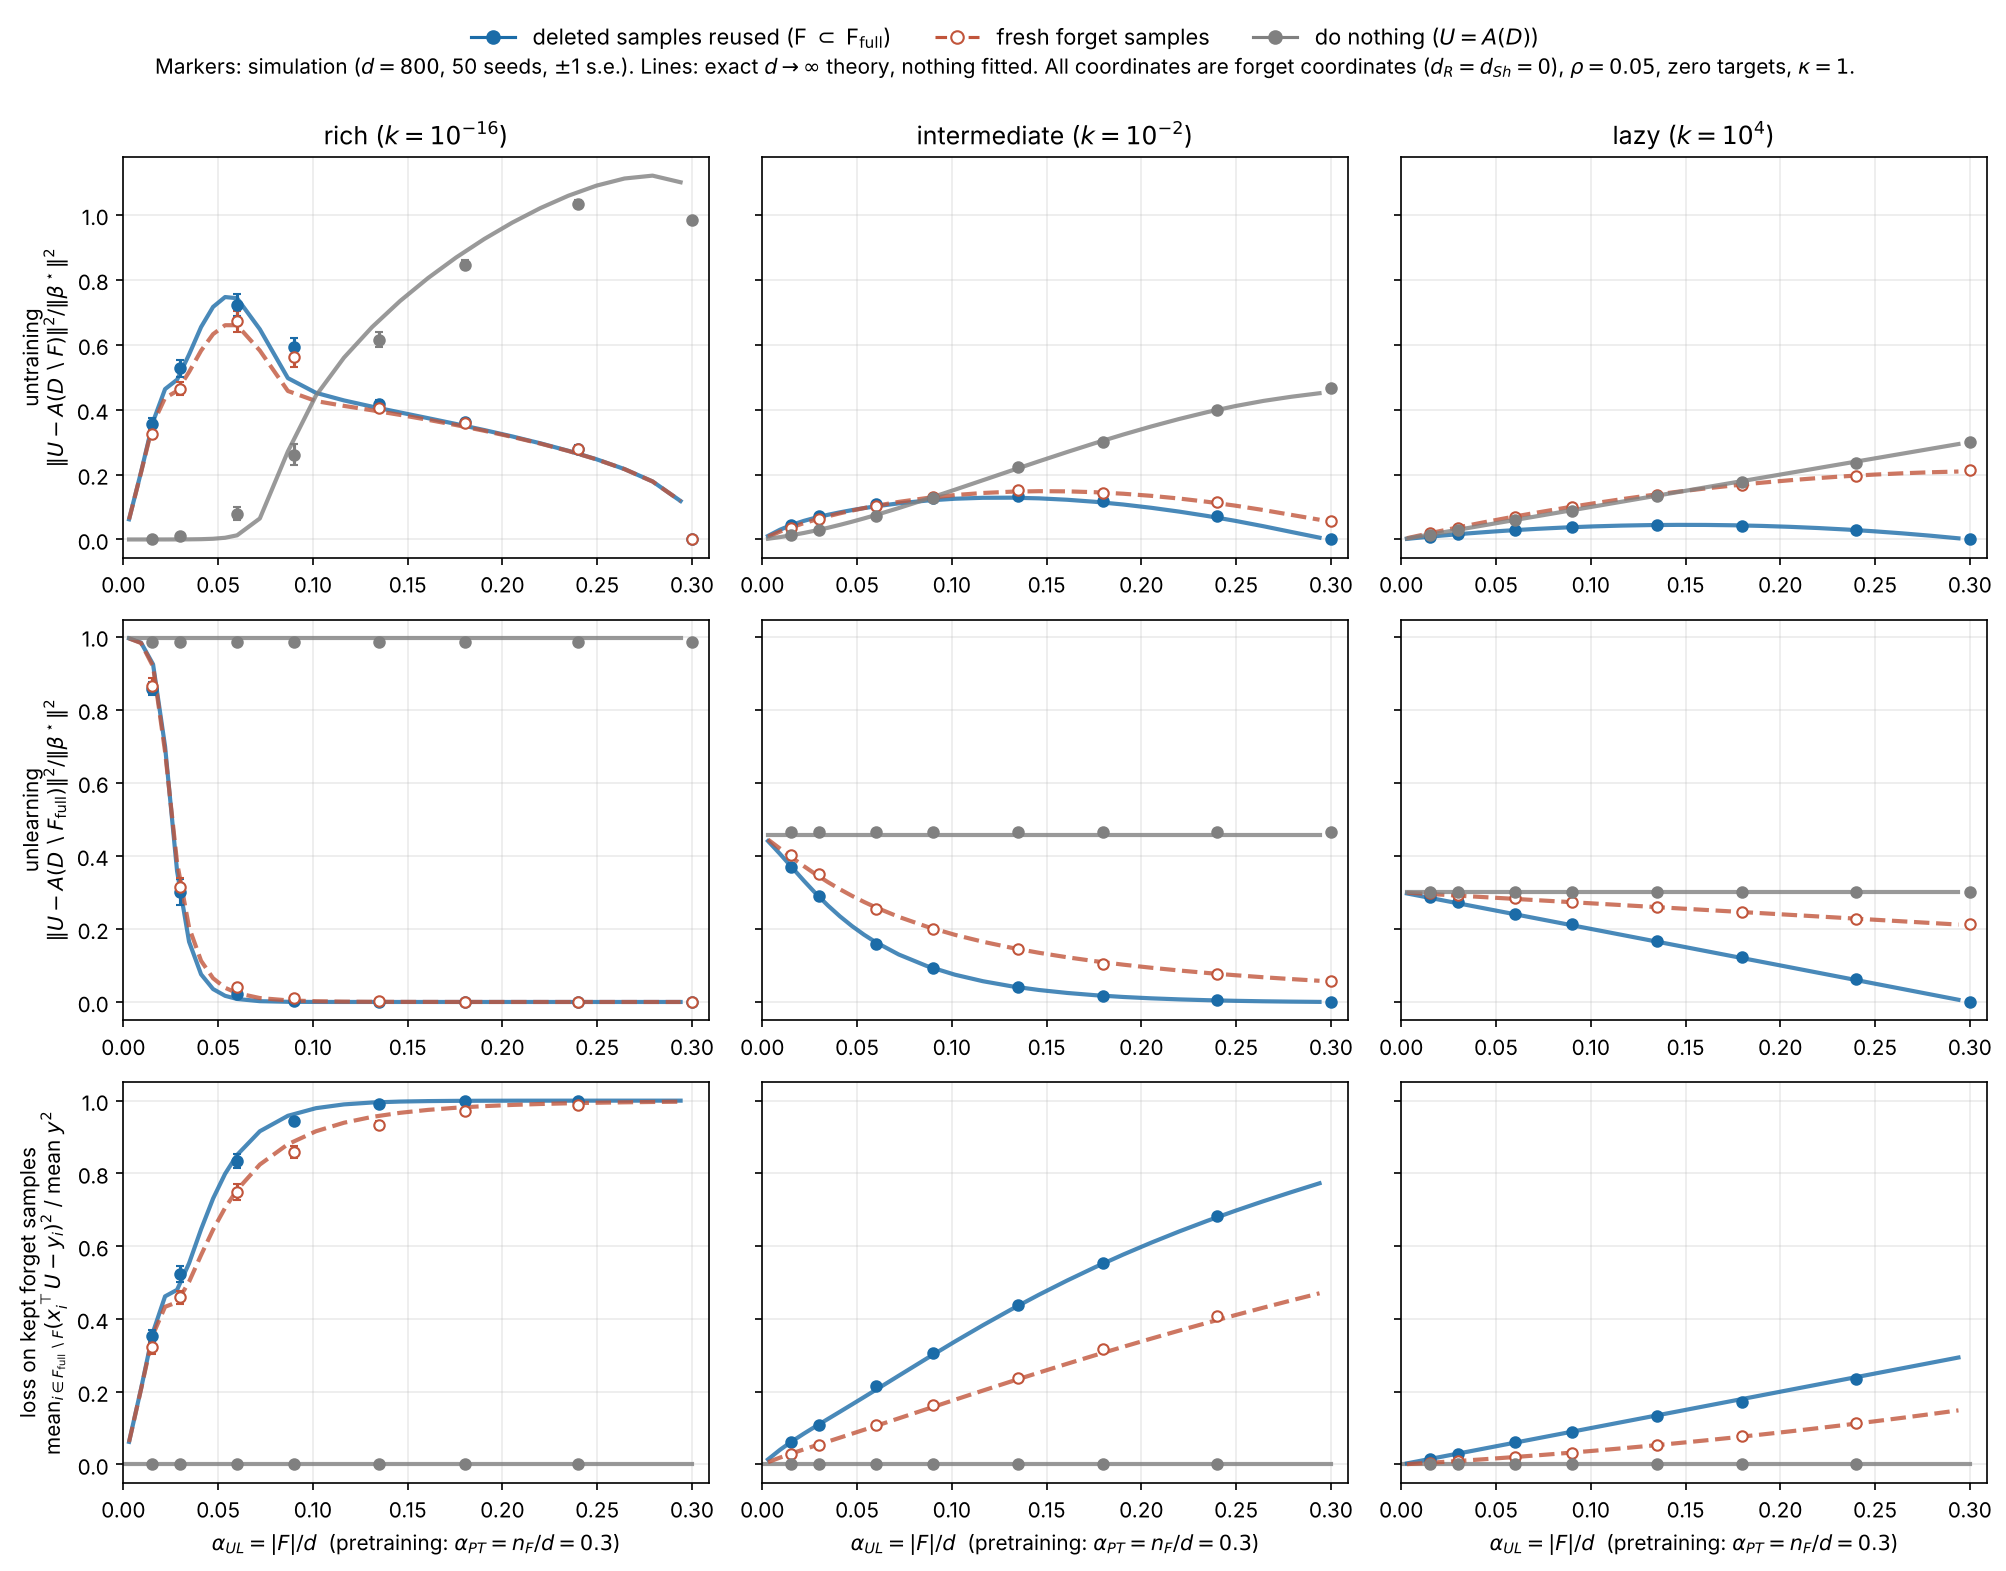
\includegraphics[width=0.93\linewidth]{fig_theory_vs_sim.png}
\caption{\small Zero targets, $\kappa=1$, forget coordinates only, $\alpha_{\mathrm{PT}}=n_F/d=0.3$, $\rho=0.05$, $d=800$, 50 seeds. Columns: rich, intermediate, lazy. Rows: distance to the untraining reference, distance to the unlearning reference, loss on the kept forget samples $\Ff\setminus F$. Blue: deleted samples reused; red: fresh samples from $P_F$; grey: do nothing. The only mismatch is the last rich untraining point: at $|F|=n_F$ the two references coincide and $A(D\setminus F)=0$, a single point the curve (computed for $|F|<n_F$) does not include.}
\end{figure}

\begin{figure}[h!]\centering
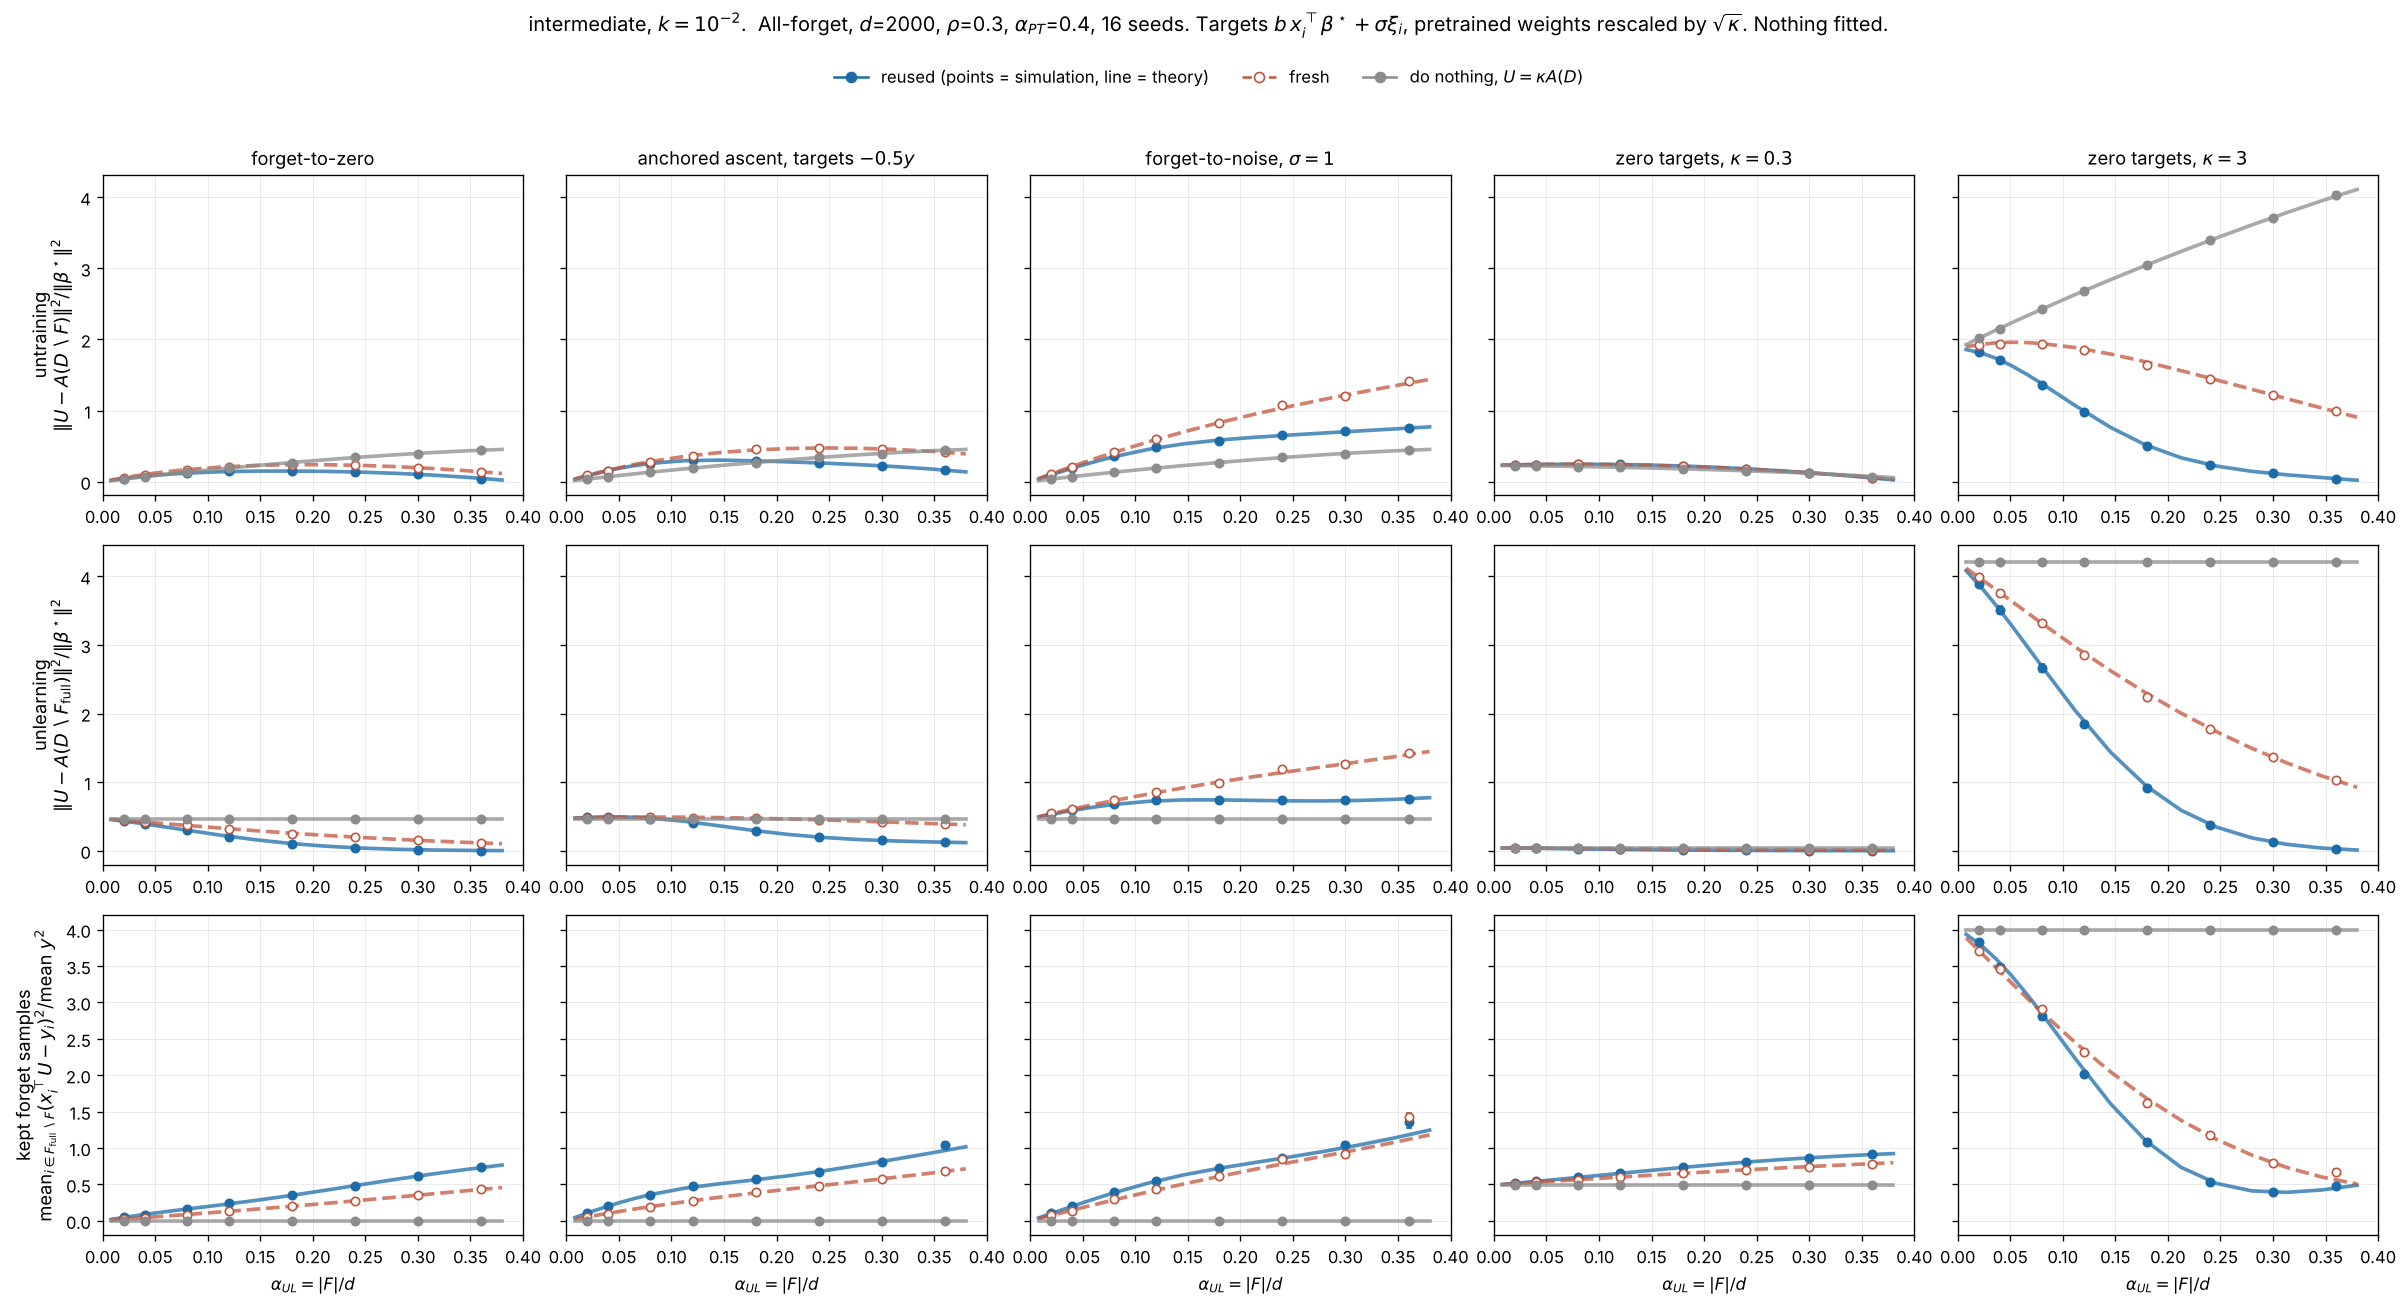
\includegraphics[width=\linewidth]{fig_losses_inter.png}
\caption{\small The same check for other stage-2 losses and rescalings, intermediate regime $k=10^{-2}$, $d=2000$, $\rho=0.3$, $\alpha_{\mathrm{PT}}=0.4$, 16 seeds. Columns: targets $0$; anchored ascent (targets $-0.5y$); targets $\sigma\xi$ (noise); targets $0$ with weights rescaled by $\sqrt\kappa$, $\kappa=0.3$ and $\kappa=3$. All losses with a fixed target reduce to the target $b\,x^\top\beta^\star+\sigma\xi$ and the starting point $\kappa A(D)$, so one theory covers them. The rich and lazy versions (\texttt{fig\_losses\_rich.png}, \texttt{fig\_losses\_lazy.png}) agree equally well.}
\end{figure}
\clearpage

\section{Results and takeaways}
Rich pretraining ($k=10^{-6}$), $\rho=0.2$, $|d_R|=|d_F|=400$, finite $d$, 6 seeds, stage 2 trained to convergence unless stated. Notation: $n_K=|\Ff\setminus F|$ kept forget samples; $\alpha_{\mathrm{DT}}(\rho)$ the recovery threshold ($0.33,\,0.51,\,0.75$ at $\rho=0.1,\,0.2,\,0.4$); $\kappa$ the rescaling of the pretrained function.

\begin{figure}[h!]\centering
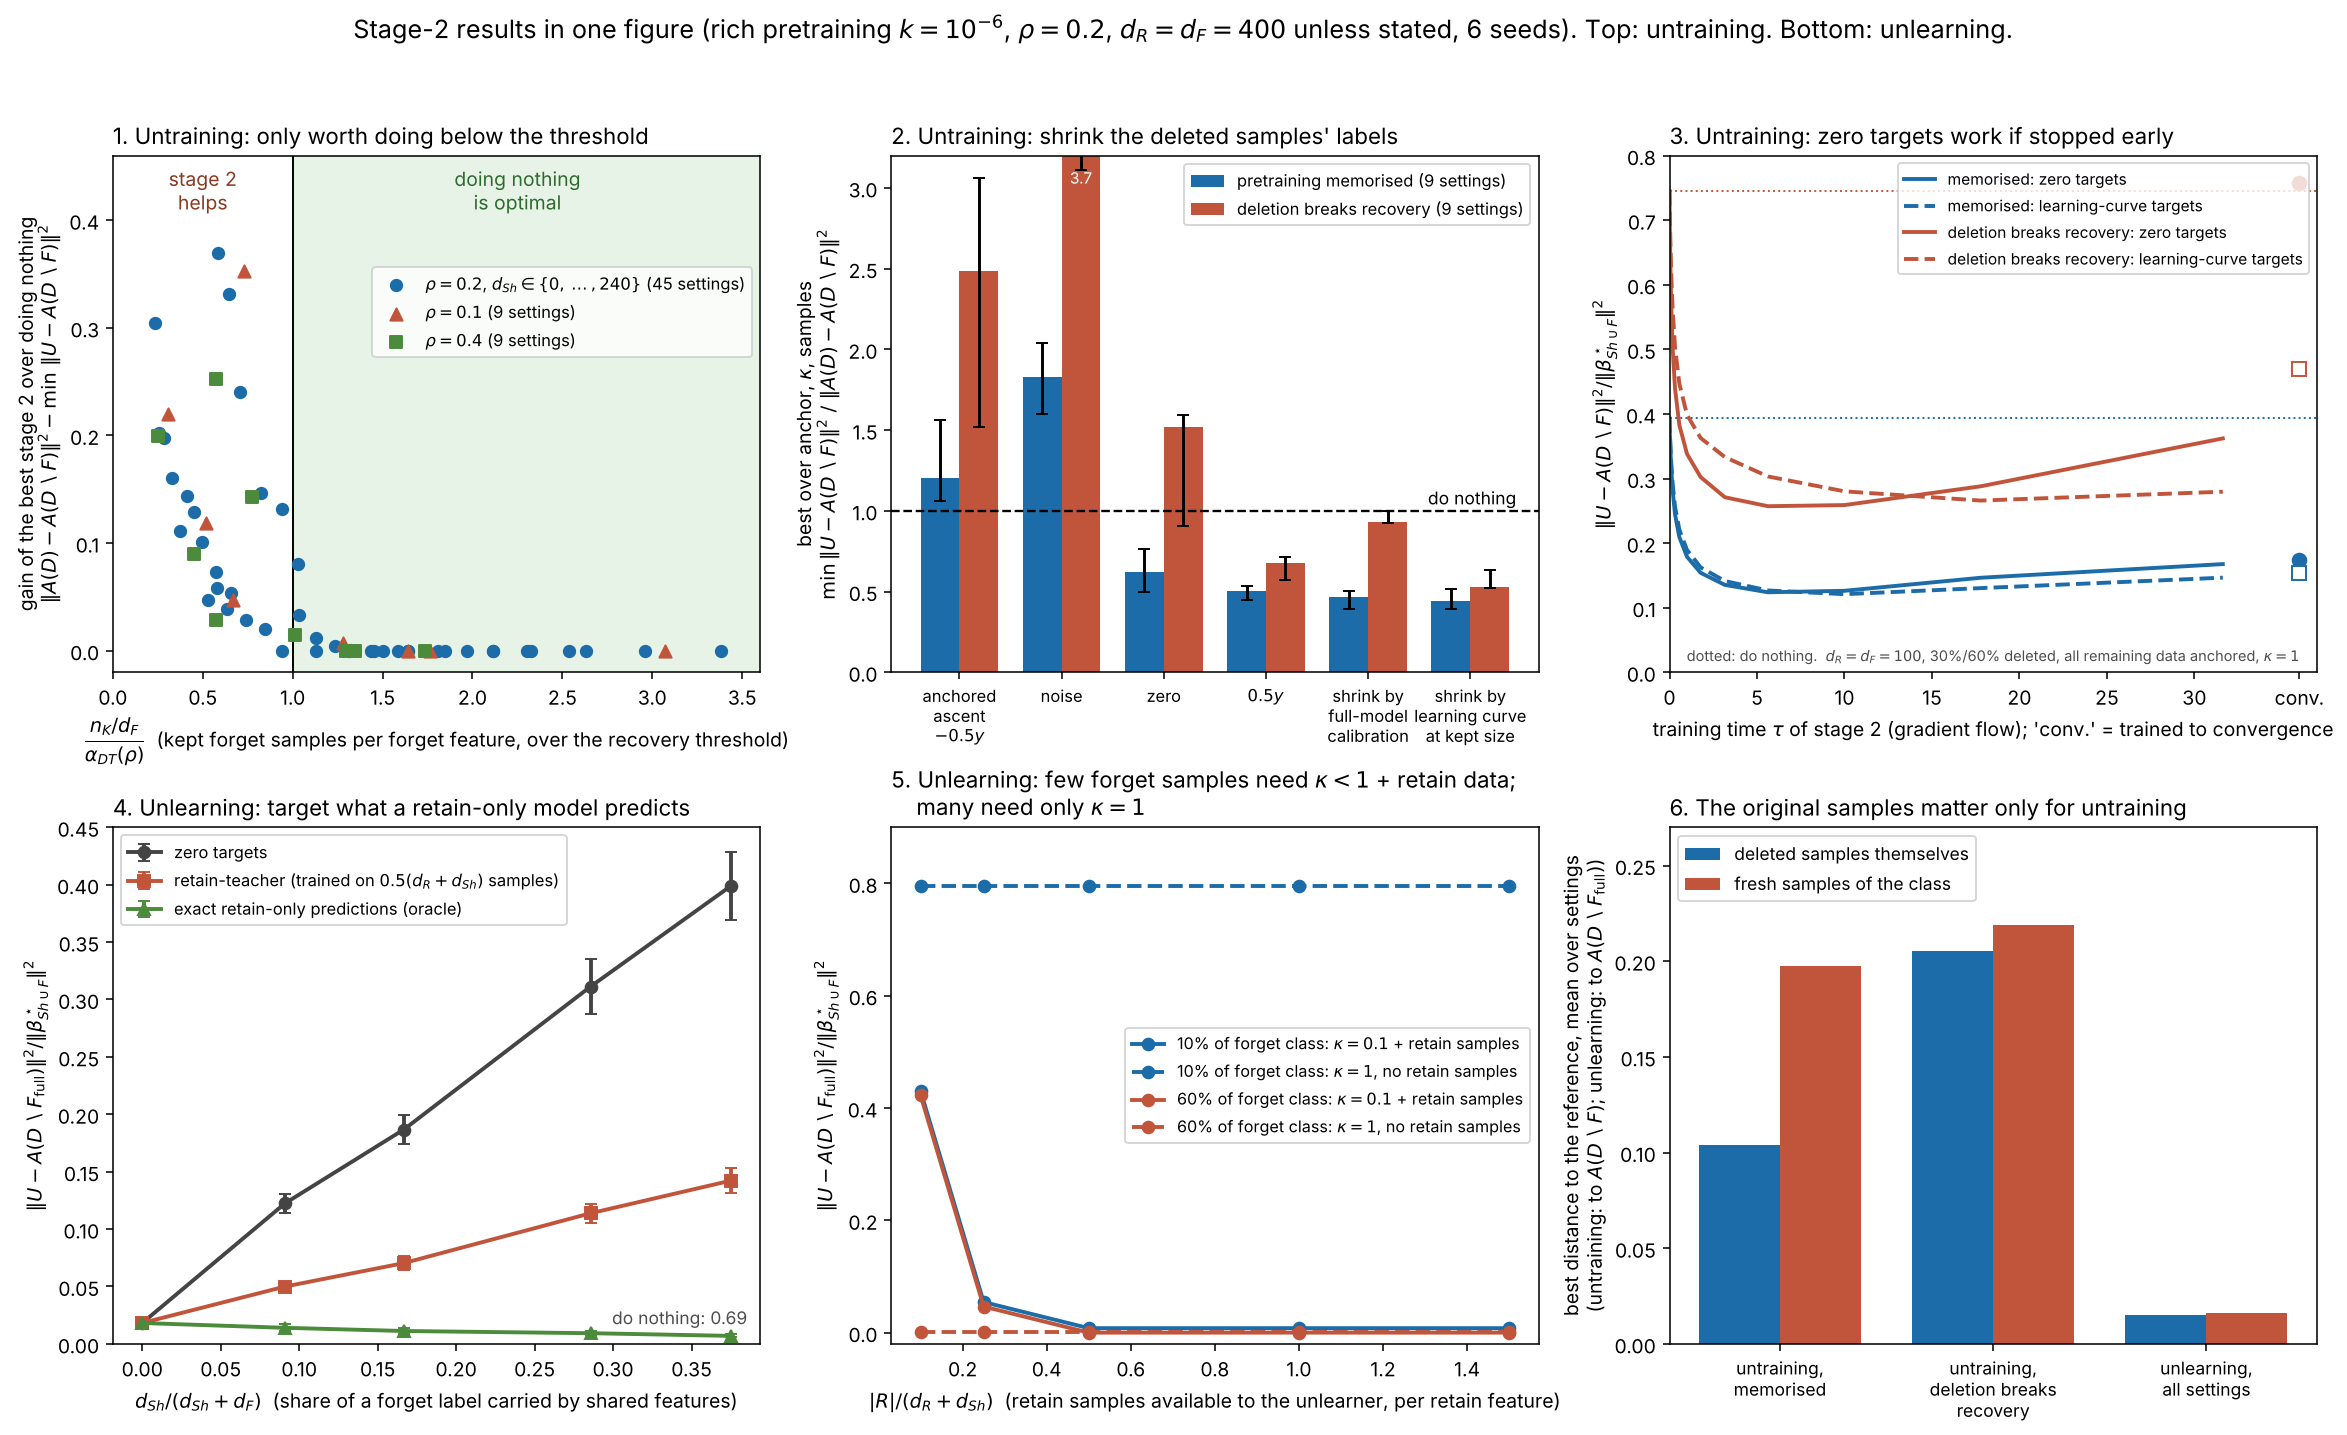
\includegraphics[width=\linewidth]{fig_results.png}
\end{figure}

\textbf{Untraining} (target $A(D\setminus F)$).
\begin{enumerate}\setlength{\itemsep}{1pt}
\item \textbf{Do nothing unless $n_K/|d_F|<\alpha_{\mathrm{DT}}(\rho)$} (panel 1). Above the threshold the kept forget data still recover $\beta^\star$, so $A(D\setminus F)=A(D)$ and any stage 2 only does harm. This held in 41/41 settings at $\rho=0.2$ and 17/17 at $\rho=0.1,0.4$.
\item \textbf{Below it, shrink the labels of the deleted samples; do not zero, invert or randomise them} (panel 2). The target $p+b\,(y-p)$, with $p$ a retain-only prediction and $b$ the learning-curve value at the kept size $n_K/|d_F|$ (from theory, no data), was best or within 1\% in 25/27 settings and 18/18 at other $\rho$. Zero targets overshoot into unlearning; ascent and noise end further from $A(D\setminus F)$ than doing nothing.
\item \textbf{Zero targets are fine if stopped early} (panel 3). With the best stopping time they match converged learning-curve targets when pretraining memorised ($0.13$ vs $0.16$) and beat them when the deletion breaks recovery ($0.26$ vs $0.47$). The stopping time can be set from the learning-curve prediction of the retrained model's held-out loss.
\item \textbf{Use the deleted samples themselves} (panel 6). After memorisation, fresh samples of the class are about twice as far from $A(D\setminus F)$ as the deleted ones, because $A(D)$ lies in the span of the samples that made it. Anchor on all remaining data; $\kappa\approx3$--$10$ helps only if every deleted sample is used. When the deletion breaks recovery, use no anchor.
\end{enumerate}

\textbf{Unlearning} (target $A(D\setminus\Ff)$).
\begin{enumerate}\setlength{\itemsep}{1pt}\setcounter{enumi}{4}
\item \textbf{Target what a model without the class would predict} (panel 4). With no shared features this is $0$; with shared features, zero targets miss by the shared part of the label (error grows linearly with $|\dSh|/(|\dSh|+|d_F|)$), and a retain-only teacher cuts the error by a factor of 3.
\item \textbf{The number of forget samples decides the recipe} (panel 5). Few forget samples ($10\%$ of $\Ff$): use $\kappa<1$ (richer) plus retain samples, at least about $0.25\,(|d_R|+|\dSh|)$ of them; $\kappa=1$ alone fails. Many ($60\%$): $\kappa=1$ and no anchor already reach $A(D\setminus\Ff)$.
\item \textbf{Reused and fresh samples are interchangeable} (panel 6), and early stopping does not help without shared features.
\end{enumerate}

\textbf{General.}
\begin{enumerate}\setlength{\itemsep}{1pt}\setcounter{enumi}{7}
\item \textbf{The loss weights $\mu_a/\mu_d$ do not matter at convergence} when every target can be fitted: the end point is a Bregman projection. They matter only when targets conflict (then the end point is a weighted least-squares fit, independent of $\kappa$) or with a finite budget.
\item \textbf{$\kappa$ moves the solution between rich ($\kappa<1$) and lazy ($\kappa>1$), but $\kappa<1$ slows training by $\kappa^2$} at a fixed budget.
\item \textbf{The theory is exact}: every curve in Section~\ref{sec:curves} matches simulation with nothing fitted, for every loss and rescaling tested.
\end{enumerate}

\textbf{Cross-entropy and the ascent losses} (added 23 Nov; forget coordinates only, $d=400$, 10 seeds, simulation unless stated).
\begin{enumerate}\setlength{\itemsep}{1pt}\setcounter{enumi}{10}
\item \textbf{With soft labels from the teacher, cross-entropy pretraining is exactly this model} (flow and projection agree to $2\times10^{-6}$). Takeaways 1--10 hold unchanged. Hard labels are not covered.
\item \textbf{Gradient ascent and NPO match the retrained model's accuracy without becoming the retrained model.} Stopped at that accuracy, their cosine to $A(D\setminus F)$ is $0.23$--$0.37$ and $0.28$--$0.54$, no better than doing nothing ($0.34$--$0.55$); the uniform target reaches $0.44$--$0.75$.
\item \textbf{Ascent inflates the logits and still carries the class.} After a relearning attack with $0.15\,d$ fresh samples its accuracy is $0.66$--$0.67$, above the retrained model's $0.61$--$0.66$.
\item \textbf{NPO stopped at chance is as hard to relearn as a model never trained on the class} ($0.585$ against $0.59$--$0.62$), though its weights are not that model's.
\item \textbf{Rescaling $\kappa$, weight decay that is switched off ($\kappa=e^{-2\Lambda}$) and mini-batch noise are the same operation} (exact; for SGD per coordinate). Weight decay kept on forgets the start instead.
\end{enumerate}

\FloatBarrier
\section{Trajectory runs with squared loss (25 November)}\label{sec:runs}
Pretraining to convergence, then unlearning for a time $\tau\le40$ by gradient descent with step $0.01$; every metric recorded along the way, with theory curves (Result 18) for $\tau\le6$. Fixed: $k=10^{-5}$, $\rho=0.2$, $d=3000$, 5 seeds. Baseline: $|d_R|:|\dSh|:|d_F|=1:0.4:1$; $0.3$ samples per coordinate seen, in each class; $|F|=\frac12|\Ff|$; $R=\Rf$; $\kappa=1$; no noise, no weight decay, full batch.

\textbf{Losses run} (names used in the figures, in the notation of Section~\ref{sec:losses}). ``Retain only'': no term on $F$. ``Forget to zero'': relabel with $\tilde\beta=0$. ``Forget to noise'': targets $\mathcal N(0,1)$ on $F$. ``Negated target $b$'': anchored ascent with $b=-\mu_a/(\mu_d-\mu_a)=-0.5,-1$. ``Signed'': gradient difference. ``Pure ascent'': the same without the retain term. In the figures ``ideal untraining'' is $A(D\setminus F)$, ``ideal unlearning'' is $A(\Rf)$, ``left-over'' samples are $\Ff\setminus F$, and the rescaling $\kappa$ is written $S$.

\textbf{Status.} Finished on all four block settings ($1:0.4:1$, $0:1:0$, $1:0:1$, $1:1:1$): baseline; $|F|/|\Ff|=0.1,0.9,1$; label noise $\sigma^2=0.1,0.5$ in pretraining; fresh forget samples; $\kappa=0.1,0.3,3$. Not run yet: loss weights, $R$ a quarter of $\Rf$, SGD, weight decay, and $0.8$ or $1.5$ samples per coordinate.

\textbf{Theory against simulation.} Relabel-to-zero and the two anchored-ascent targets: 2868 comparisons, $94\%$ within 2 standard errors, median gap $3.0\%$ (Figure~\ref{fig:base}). Targets of noise are much noisier (the outcome follows the empirical variance of the $\approx260$ noise targets); with 12 runs per side they agree, except a $\approx10\%$ excess of theory on the kept forget samples for $\tau\ge4$ (Figure~\ref{fig:noise}). Gradient difference: theory predicts no motion (Result 10); in simulation it diverges at $\tau\approx2$--$4$ from the $2\times10^{-4}$ training error left by pretraining.

\begin{figure}[!ht]\centering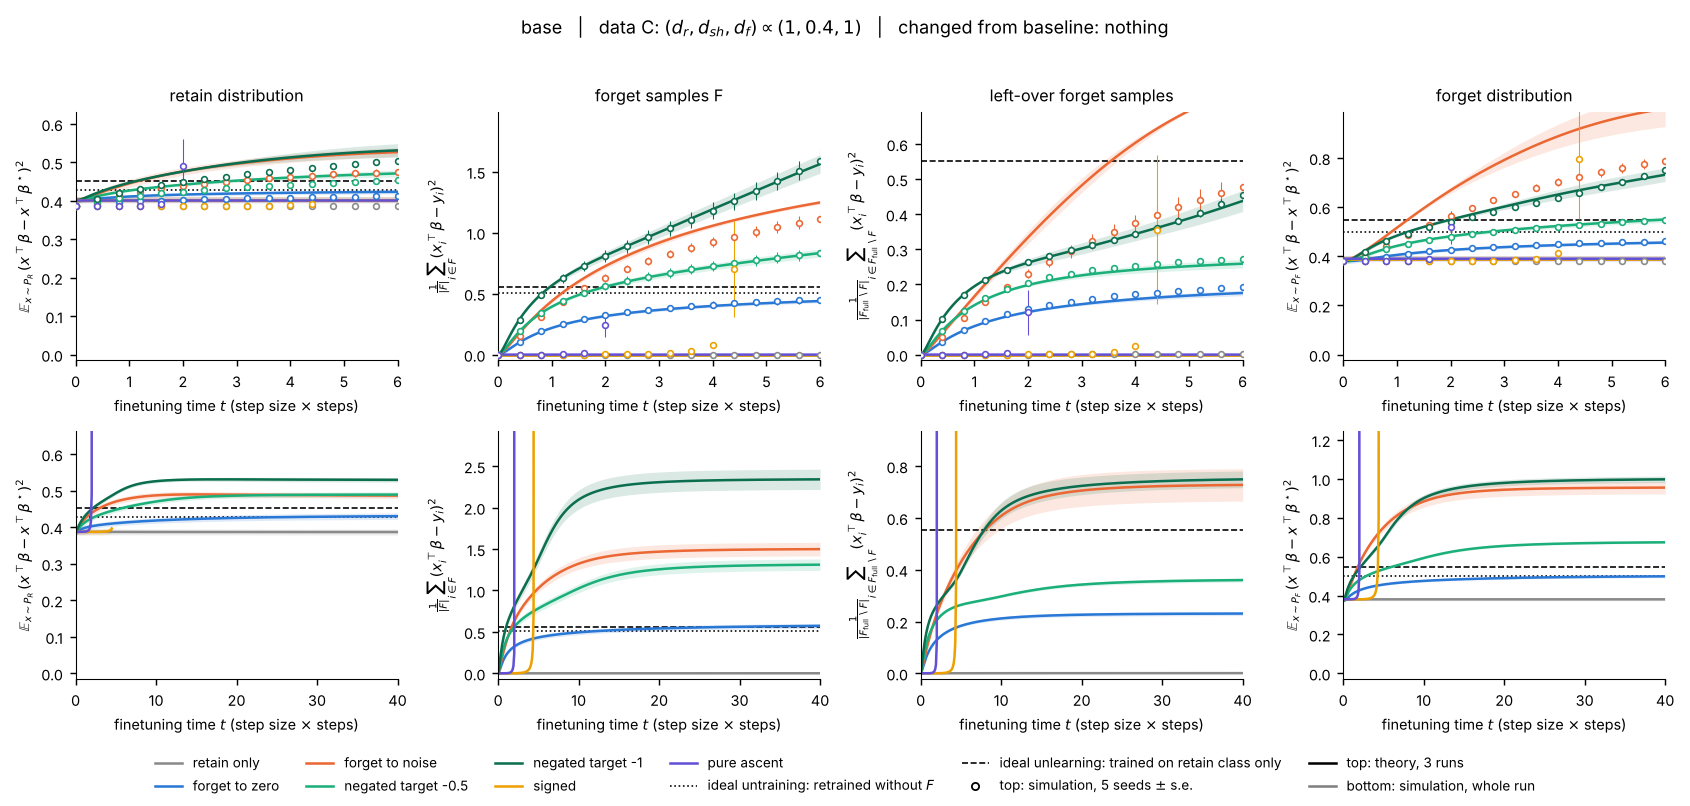
\includegraphics[width=\linewidth]{figs/base__C.png}
\caption{\small Baseline. Top: theory (lines) and simulation (markers) for $\tau\le6$. Bottom: simulation to $\tau=40$. The orange theory curve (targets of noise) is three unlucky runs; see Figure~\ref{fig:noise}.}\label{fig:base}\end{figure}
\begin{figure}[!ht]\centering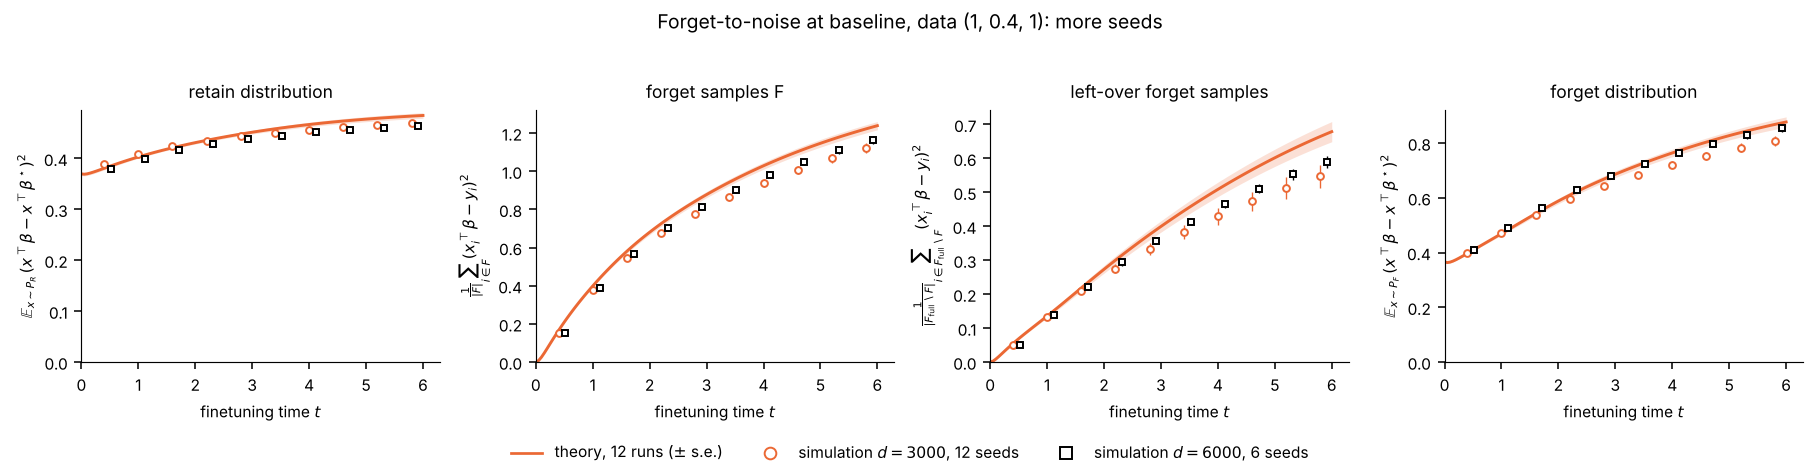
\includegraphics[width=\linewidth]{figs/noise_more_seeds.png}
\caption{\small Targets of noise at baseline with 12 runs per side.}\label{fig:noise}\end{figure}

\textbf{Baseline, end of unlearning} (simulation).
\begin{center}\small\begin{tabular}{@{}lcccccc@{}}\toprule
& retain error & error on $F$ & on $\Ff\setminus F$ & forget error & dist.\ to $A(D\setminus F)$ & dist.\ to $A(\Rf)$\\\midrule
$A(D)$ & 0.387 & 0.000 & 0.000 & 0.381 & 0.207 & 0.290\\
$A(D\setminus F)$ & 0.429 & 0.507 & 0.000 & 0.499 & 0 & \\
$A(\Rf)$ & 0.452 & 0.555 & 0.553 & 0.547 & & 0\\\midrule
relabel to $0$ & 0.430 & 0.573 & 0.231 & 0.499 & 0.140 & 0.096\\
anchored ascent, $b=-0.5$ & 0.489 & 1.311 & 0.360 & 0.674 & 0.260 & 0.249\\
anchored ascent, $b=-1$ & 0.530 & 2.341 & 0.749 & 0.998 & 0.530 & 0.567\\
targets of noise & 0.486 & 1.499 & 0.727 & 0.955 & 0.657 & 0.736\\\bottomrule
\end{tabular}\end{center}
Smallest distance along the path (time reached), to $A(D\setminus F)$ and to $A(\Rf)$: relabel to $0$, $0.119$ ($\tau=2.3$) and $0.090$ ($11.7$); $b=-0.5$: $0.125$ ($0.8$) and $0.112$ ($2.2$); $b=-1$: $0.129$ ($0.4$) and $0.127$ ($0.9$). Anchored ascent passes near the same point 3--5 times sooner, then overshoots.

\textbf{Blocks} (relabel to $0$).
\begin{center}\small\begin{tabular}{@{}lcccc@{}}\toprule
$|d_R|:|\dSh|:|d_F|$ & $1:0:1$ & $1:0.4:1$ & $1:1:1$ & $0:1:0$\\\midrule
retain error, $A(D)\to$ end & $0.374\to0.374$ & $0.387\to0.430$ & $0.356\to0.472$ & $0.068\to0.704$\\
distance to $A(\Rf)$, start $\to$ end & $0.222\to0.012$ & $0.290\to0.096$ & $0.339\to0.187$ & $0.523\to0.395$\\
distance to $A(D\setminus F)$, start $\to$ best & $0.184\to0.094$ & $0.207\to0.119$ & $0.221\to0.135$ & $0.262\to0.196$\\\bottomrule
\end{tabular}\end{center}
With no shared block the retain error does not move (Result 9) and relabel-to-zero converges to $A(\Rf)$. With all coordinates shared, both classes together exceed the recovery threshold, $A(D)$ is nearly $\beta^\star$, and every forget loss destroys the retain error.

\begin{figure}[!ht]\centering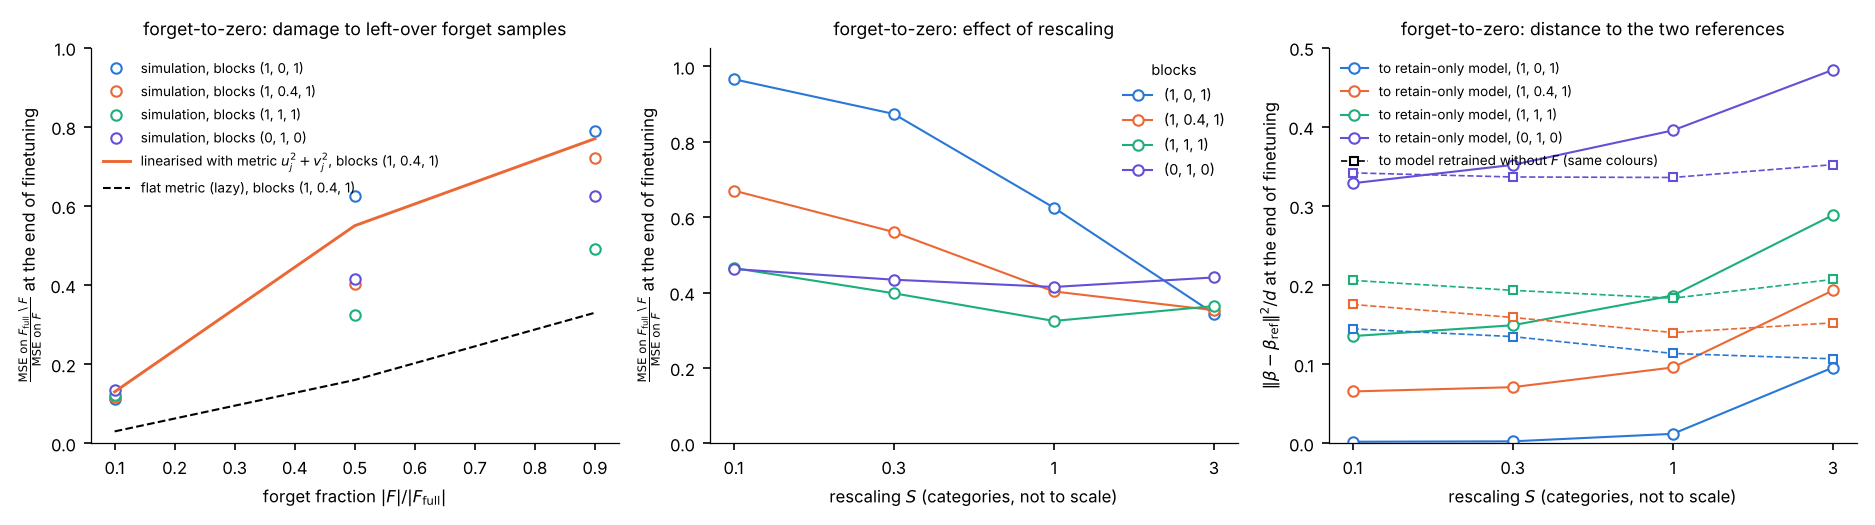
\includegraphics[width=\linewidth]{figs/summary.png}
\caption{\small Relabel to $0$ at the end of unlearning. Left: error on $\Ff\setminus F$ relative to error on $F$, against $|F|/|\Ff|$. Middle and right: against the rescaling $\kappa$ (written $S$).}\label{fig:sum}\end{figure}

\textbf{Deletion size} (Figure~\ref{fig:sum}, left). The ratio (error on $\Ff\setminus F$)/(error on $F$) is $0.12,0.40,0.72$ at $|F|/|\Ff|=0.1,0.5,0.9$; the local rule (Result 7) gives $0.13,0.55,0.77$, a flat metric $0.03,0.16,0.33$.

\textbf{Rescaling} (Figure~\ref{fig:sum}, middle and right). Larger $\kappa$ lowers the damage to the kept forget samples and raises the distance to $A(\Rf)$; smaller $\kappa$ does the opposite. Blocks $1:0:1$: ratio $0.97,0.87,0.63,0.34$ and distance to $A(\Rf)$ $0.002,0.002,0.012,0.096$ at $\kappa=0.1,0.3,1,3$, as the corollary of Result 4 predicts.

\textbf{Label noise in pretraining.} All errors rise; the ratio above stays $0.40$ at $\sigma^2=0.1$; the ordering of losses is unchanged. \textbf{Fresh forget samples.} Relabel-to-zero on fresh samples raises the error on $F$ and on $\Ff\setminus F$ equally ($0.143$, $0.137$): it cannot single out $F$; the distance to $A(\Rf)$ ends at $0.197$ (reused: $0.096$).

\FloatBarrier
\section{Extensions (24 November)}
Checks and proofs for the cross-entropy items are in \texttt{extensions\_maths.pdf}; this is the list.
\begin{enumerate}\setlength{\itemsep}{1pt}
\item \textbf{Stage 2 with retain, shared and forget blocks is exact at large $d$.} Pretrained, unlearned and both retrained models are coupled copies of one static system; anchors and any $\kappa$ included. 26 distances within 1.8 s.e.
\item \textbf{Cross-entropy.} Soft labels are the squared-loss model. Hard labels: exact end point with weight decay kept on; without it there is no end point and the exact object is the trajectory.
\item \textbf{Ascent, NPO, flipped labels, task vector, WHP} on hard labels follow the same trajectory equations. Ascent improves the cosine to the retrained model after hard-label pretraining ($0.55\to0.75$) and not after soft-label pretraining ($0.52\to0.53$).
\item \textbf{Early stopping at a fixed budget} ($k=10^{-2}$): short stage 2, overshooting targets $-0.5y$ with an anchor; long stage 2, zero targets with an anchor.
\item \textbf{SGD} is a rescaling $\kappa_j$ per coordinate; its large-$d$ trajectory is exact at any step and batch size, in both stages.
\item \textbf{Weight decay switched off is a rescaling}, $\kappa=e^{-2\Lambda}$; kept on, the end point is a lasso and forgets the start.
\item \textbf{Proved:} the trajectory equations for the truncated network, with a sharp switch and hard labels. \textbf{Open:} removing the truncation; non-convex penalties.
\end{enumerate}

\section{What is and is not derived}
\begin{center}\small\begin{tabular}{@{}p{7.5cm}p{7.5cm}@{}}\toprule
derived & not derived\\\midrule
Results 1--12: exact (Result 5 assumes the flow reaches the stationary point) & why the distance to $A(D\setminus F)$ never falls below about half its starting value\\
Results 13--16: replica, assuming replica symmetry and the saddle point; end points agree with simulation (tables in Sections~\ref{rep2}--\ref{sec:refs}) & a closed formula for the spread in the rich regime beyond the first-order rule \eqref{lin} (about $1.3\times$ too high at large $|F|$)\\
Results 17--19: cavity; trajectories agree with simulation ($94\%$ of 2868 comparisons within 2 standard errors) & oracle targets; the attacker's stage; unlearning after SGD pretraining; end points when the targets cannot all be fitted\\\bottomrule
\end{tabular}\end{center}
\section{Plan}
Compute $\alpha_{\mathrm{UL}}$, $\alpha_{\mathrm{UT}}$ and $\alpha_{\mathrm{re}}$ over a grid of $\mu_a/\mu_d$ (loss), $k$ and $\kappa$ (geometry) and $|\Ff|/|d_F|$ (data), with weight decay as the deletion baseline. Repeat at finite stopping times $\tau$: in closed form in the lazy regime, and by gradient flow elsewhere, recording the readiness of the $d_F$ coordinates alongside $\alpha_{\mathrm{re}}$.


\end{document}
